\documentclass[aspectratio=169]{beamer}
% \documentclass{beamer}

\usetheme{metropolis}
\usepackage[T1]{fontenc}
\usepackage{microtype}
\usepackage{booktabs}
\usepackage{float}
\usepackage{amsmath}
\usepackage{mathtools}
\usepackage{graphicx}
\usepackage{tabularray}
\usepackage{amssymb}
\usepackage{csquotes}
\usepackage{adjustbox}
\usepackage{hyperref}
\usepackage{listings}
\usepackage{xcolor}
\usepackage[justification=centering]{caption}

% --- Bibliography setup ---
\usepackage[
  backend=biber,
  style=authoryear,
  maxcitenames=2,
  uniquename=false,
  giveninits=true
]{biblatex}

\lstset{language=SQL,morekeywords={PREFIX,java,rdf,rdfs,url}}

\addbibresource{references/references.bib}
\title{SolidSessionBench: Realistic Query Sequences for User-Oriented Decentralized Environments}
\date{\today}
\author{Ruben Eschauzier, Ruben Taelman}
\institute{Department of Electronics and Information Systems, Ghent University – Imec}

\begin{document}

\maketitle

% NOTES:
%   - Table of Contents and come back to it
% So like a agenda that shows up every once in a while
% Something like: The goal of the paper and why, new tools for our analysis, the experiment run, results

% NOTES:
% (DONE)
%   Take more time to justify why decentralized environments, the use-case is good but:
%       - Mention how its only one of the use-cases (check)
%       - Explain it more how decentralized matters with more anecdotes (check)
%       - Transition from centralized to link traversal doesn't make any goddamn sense (check)
%       - Why do we use documents? Why not sparql endpoints? Documents are very unexpressive allowing flexible data representation without large server cost.
%       - User in the loop privacy controls instead of granular, once data is in centralized storage its difficult to get it out.
%       - Maybe remove the slide talking about centralized querying
%       - Document serving of resources is less expressive (can answer less types of questions, just what is in the document)
%         becomes less expensive per level of granularity fine-grained access control

% \begin{frame}{The Motivation for Decentralized Personal Data Storage}
%     \begin{columns}[T] % T aligns columns at the top
%         % Left column: Image
%         \begin{column}{0.6\textwidth} % Adjust width as needed
%             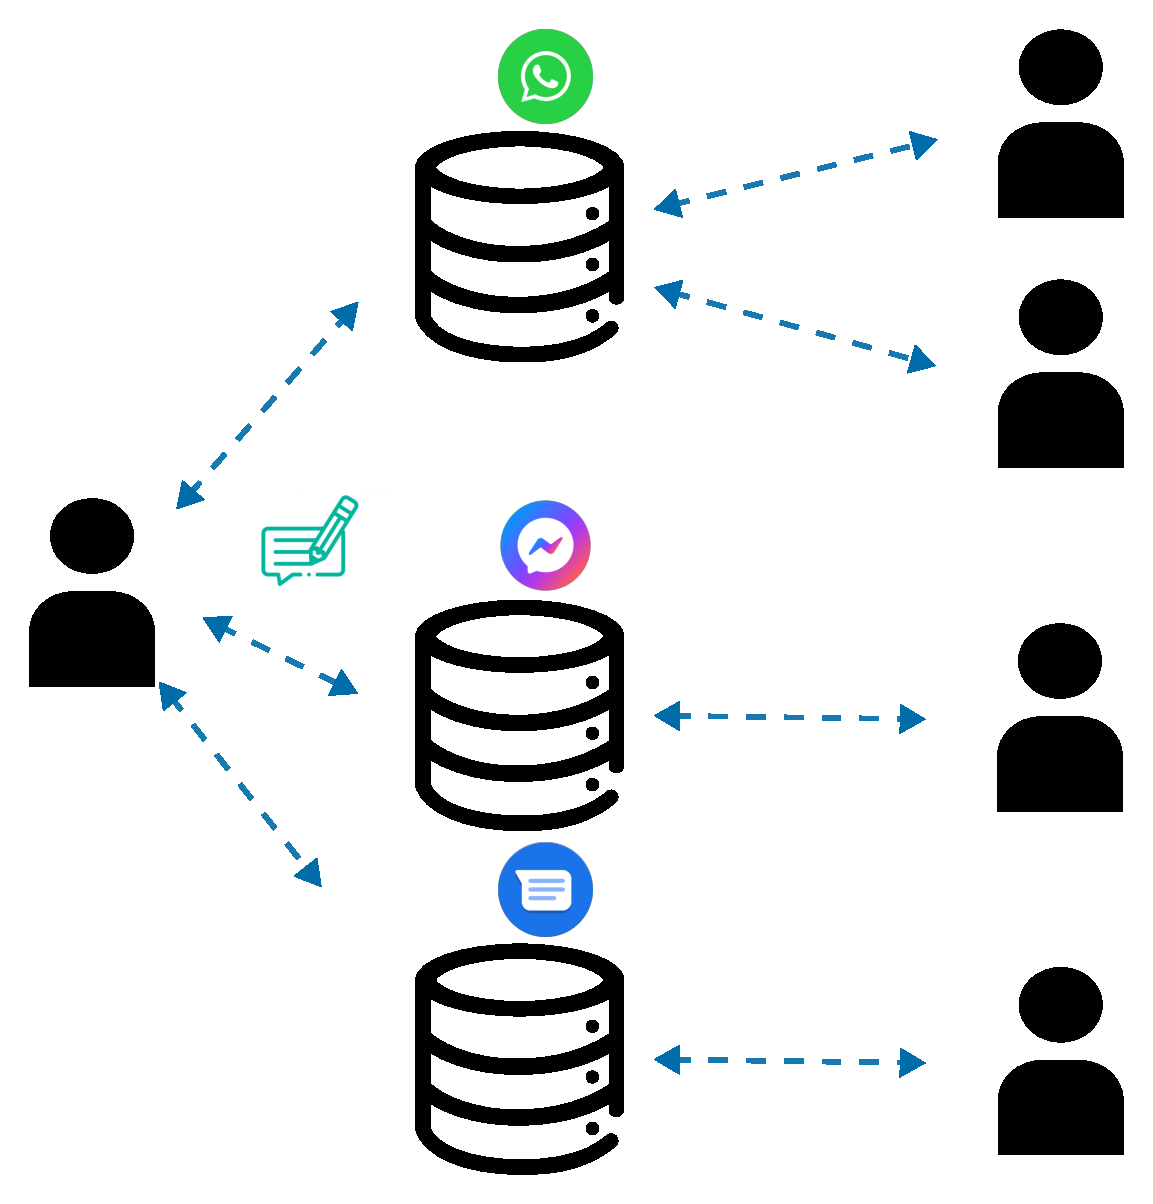
\includegraphics[width=.85\linewidth]{images/current-bad-message-situation.pdf} % replace with your image file
%         \end{column}

%         % Right column: Text
%         \begin{column}{0.4\textwidth} % Adjust width as needed
%             \begin{itemize}
%                 \item Each application has its own data
%                 \item Stifles innovation
%                 \item Causes vendor lock-in
%             \end{itemize}
%         \end{column}
%     \end{columns}
% \end{frame}
\begin{frame}{The Motivation for Decentralized Personal Data Storage}
    \begin{columns}
        \begin{column}{0.6\textwidth}
            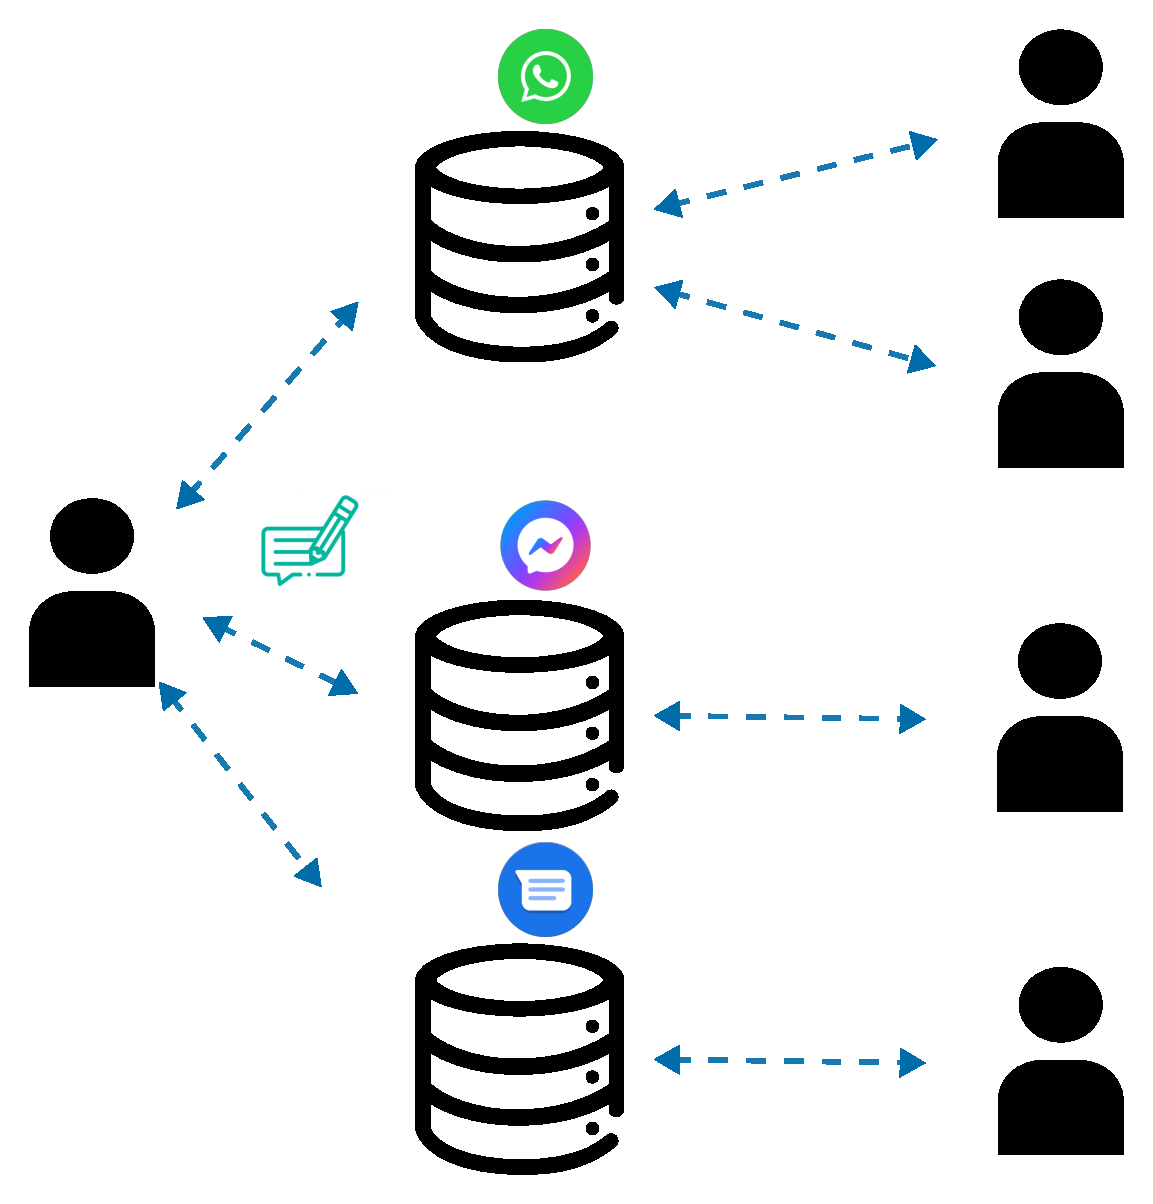
\includegraphics[width=.85\linewidth]{images/current-bad-message-situation.pdf}
        \end{column}

        \begin{column}{0.4\textwidth}
            \begin{itemize}\setlength\itemsep{1em} % <-- added spacing here
                \item Each application has its own data
                \item Stifles innovation
                \item Causes vendor lock-in
            \end{itemize}
        \end{column}
    \end{columns}
\end{frame}

\begin{frame}{The Motivation for Decentralized Personal Data Storage}
    \begin{columns}[T] % T aligns columns at the top
        % Left column: Image
        \begin{column}{0.6\textwidth} % Adjust width as needed
            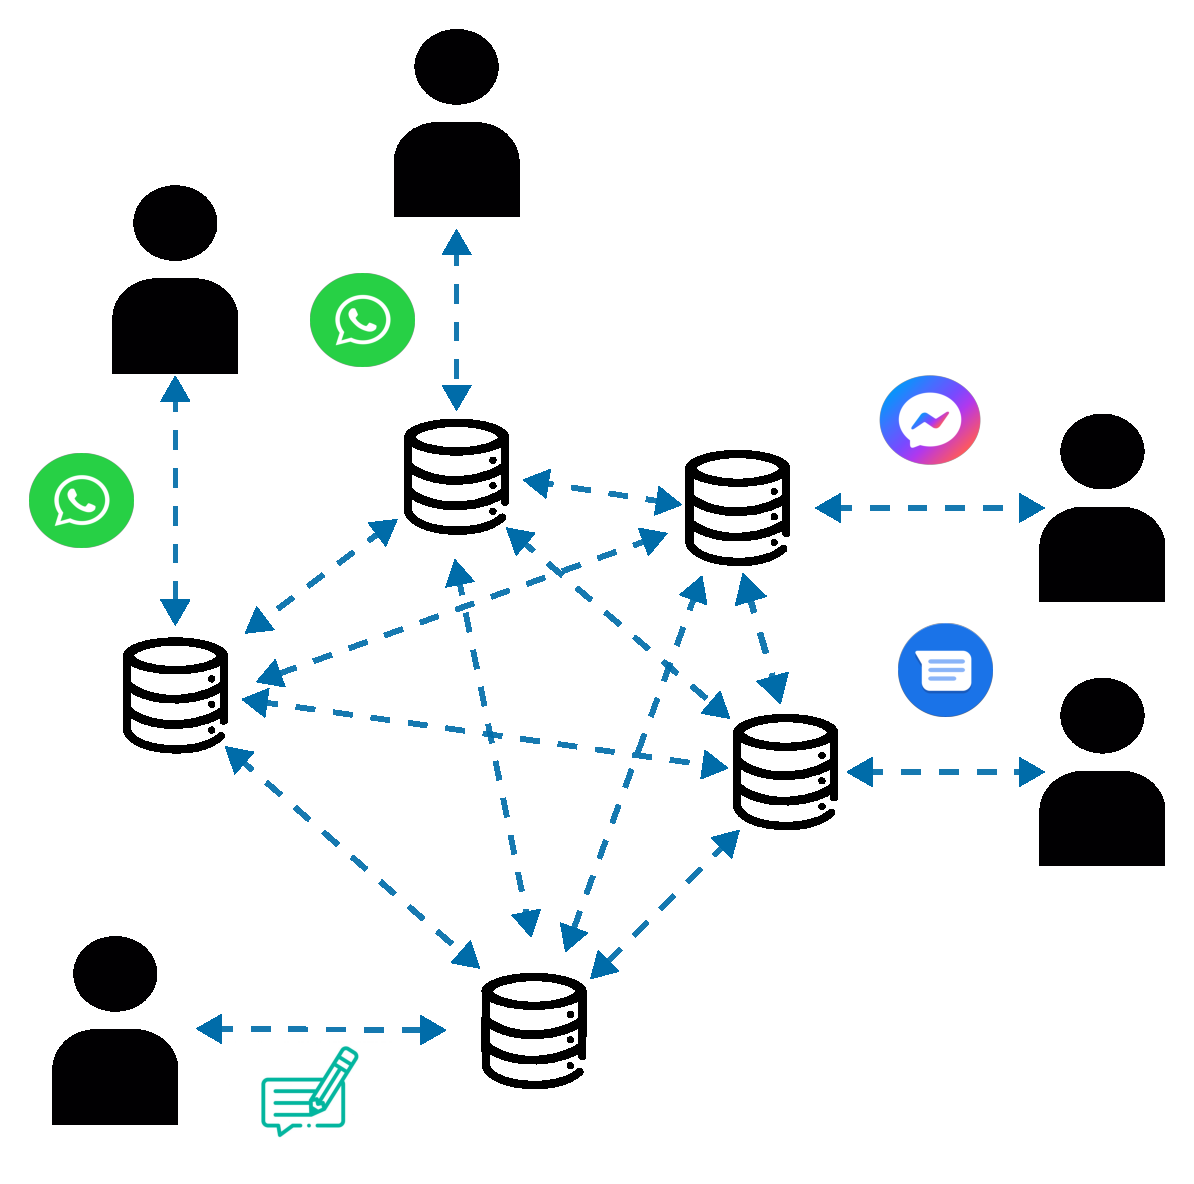
\includegraphics[width=.9\linewidth]{images/decentralized-message-storage.pdf} % replace with your image file
        \end{column}

        % Right column: Text
        \begin{column}{0.4\textwidth} % Adjust width as needed
            \begin{itemize}
                \item Each application accesses a common decentralized data environment
                \item Easy to switch vendors
                \item Promotes innovation
            \end{itemize}
        \end{column}
    \end{columns}
\end{frame}

\begin{frame}{Querying Structured Decentralized Environments}
    \begin{columns}[T] % T aligns columns at the top
        % Left column: Image
        \begin{column}{0.6\textwidth} 
            \centering% Adjust width as needed
            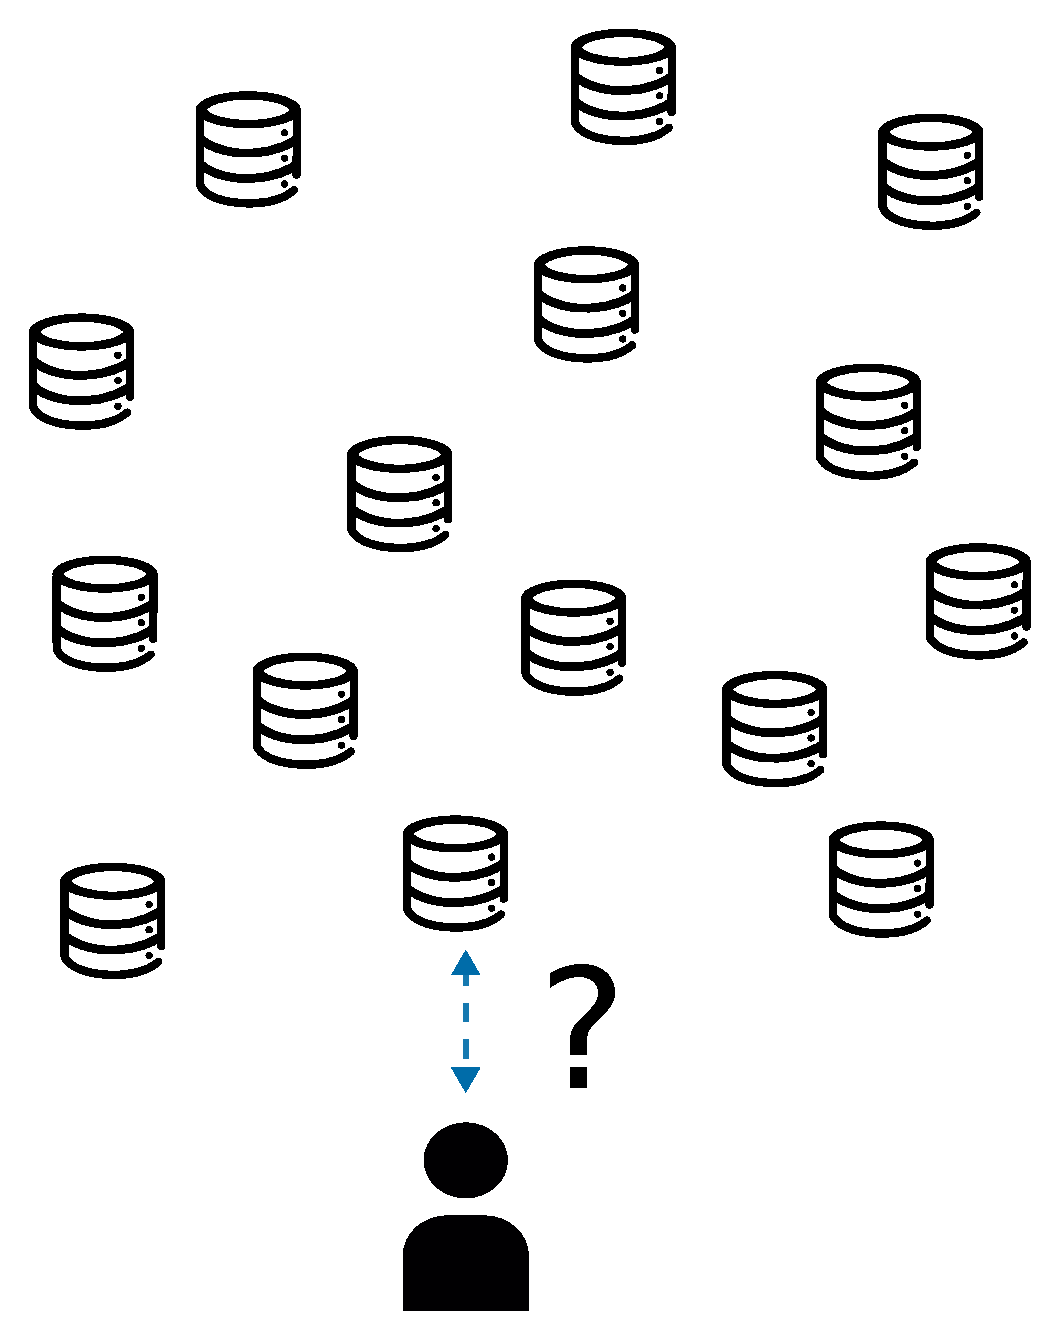
\includegraphics[width=.6\linewidth]{images/how-to-find-sources.pdf} % replace with your image file
        \end{column}

        % Right column: Text
        \begin{column}{0.4\textwidth} % Adjust width as needed
            \begin{itemize}
                \item How do we discover and query these sources?
            \end{itemize}
        \end{column}
    \end{columns}
\end{frame}
% \begin{frame}{The Problem with Centrally Aggregating and Querying}
%     \begin{columns}[T] % T aligns columns at the top
%         % Left column: Image
%         \begin{column}{0.6\textwidth} % Adjust width as needed
%             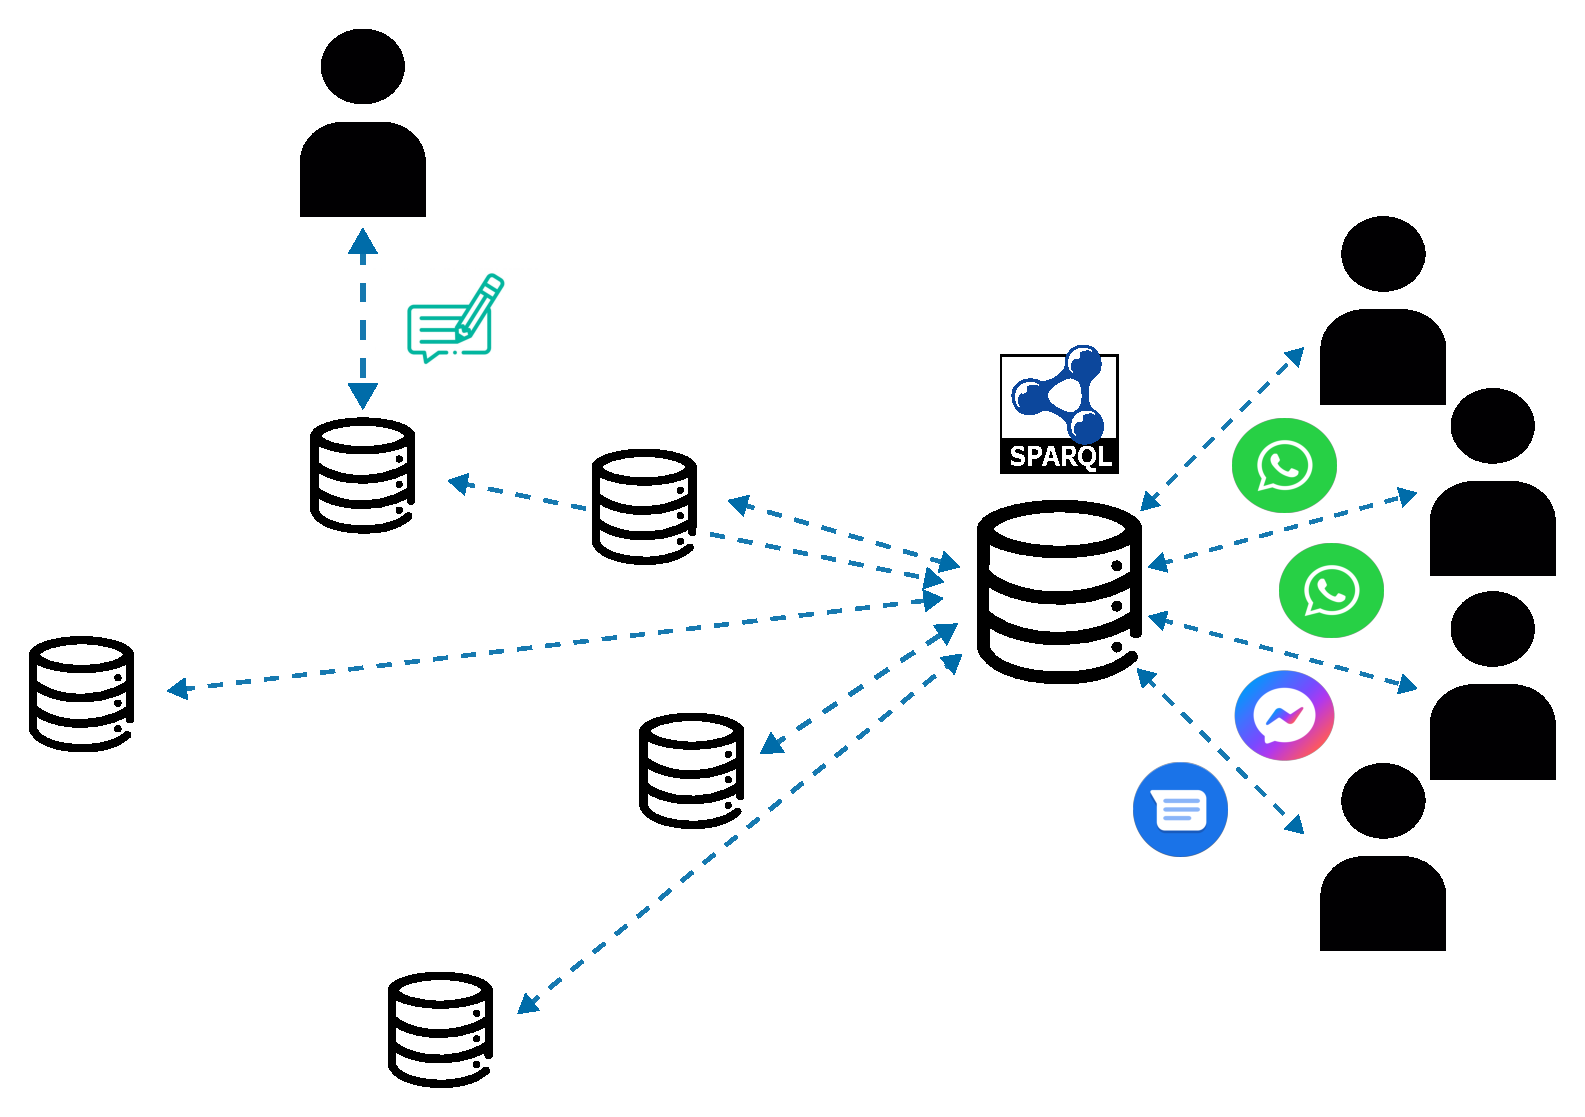
\includegraphics[width=\linewidth]{images/centralize-personal-data-stores.pdf} % replace with your image file
%         \end{column}

%         % Right column: Text
%         \begin{column}{0.4\textwidth} % Adjust width as needed
%             \begin{itemize}
%                 \item Why not aggregate data and query it?
%                 \item Difficult in case of personal data due to privacy concerns
%             \end{itemize}
%         \end{column}
%     \end{columns}
% \end{frame}

% \begin{frame}{The Problem with Centrally Aggregating and Querying}
%     \begin{columns}[T] % T aligns columns at the top
%         % Left column: Image
%         \begin{column}{0.6\textwidth} % Adjust width as needed
%             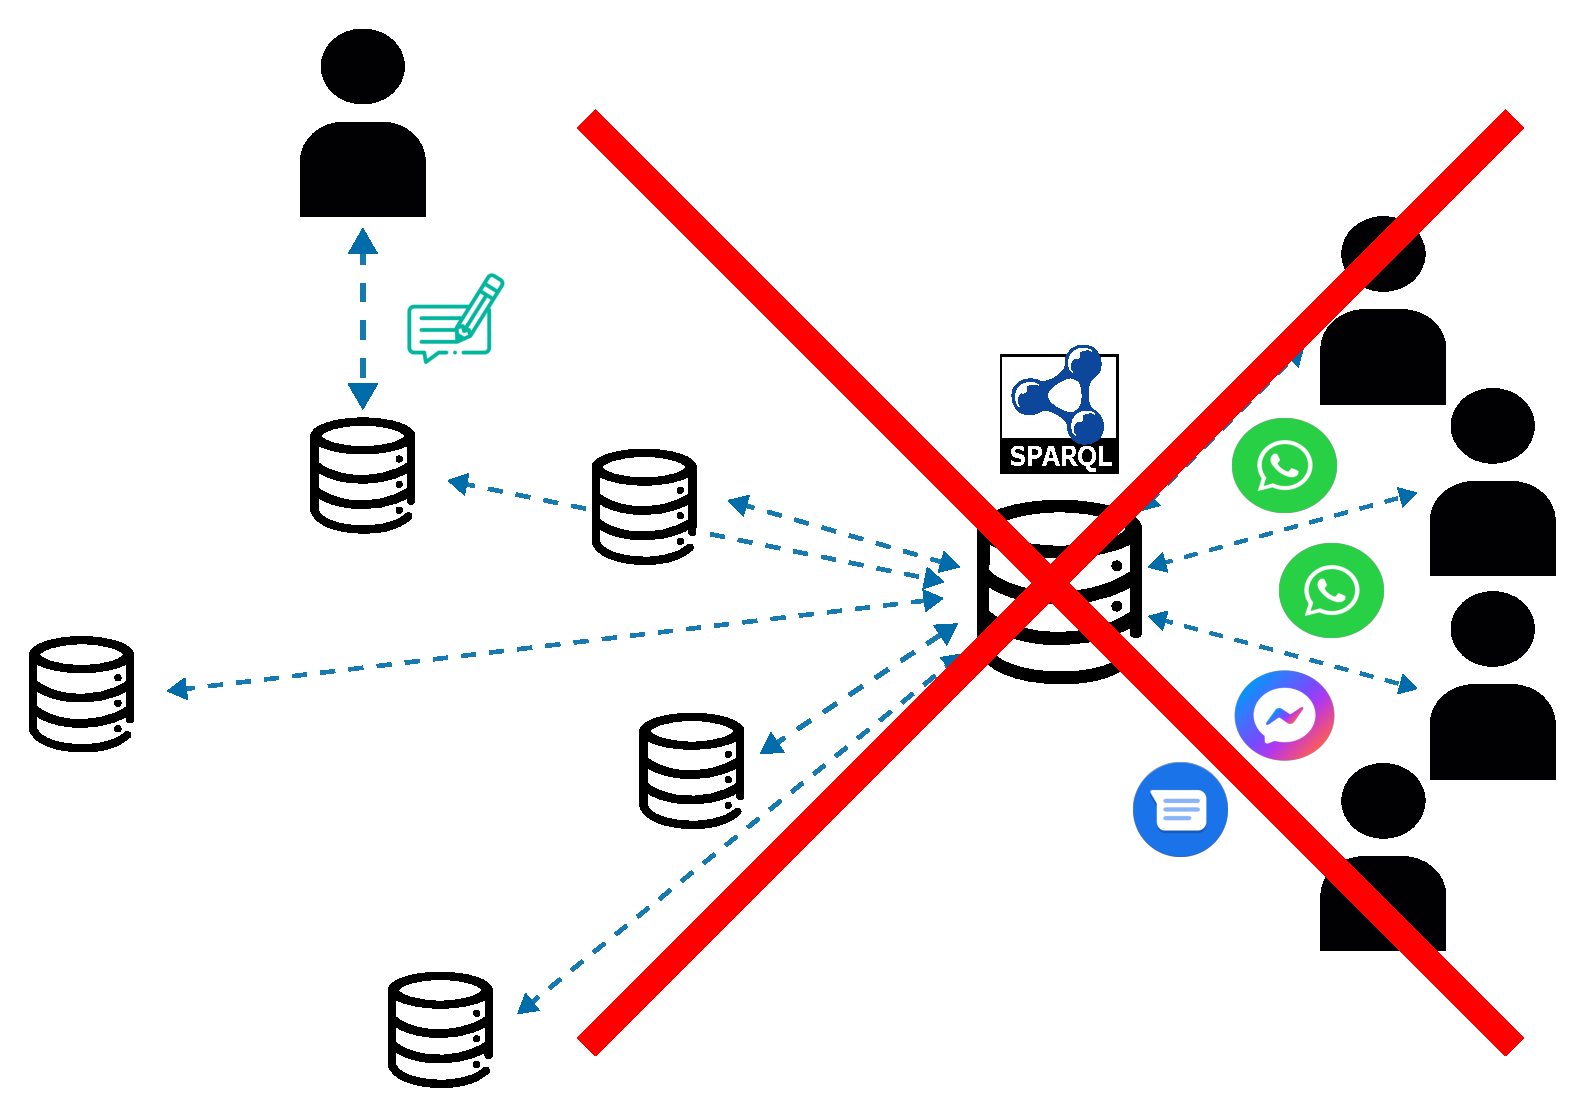
\includegraphics[width=\linewidth]{images/centralize-personal-data-stores-no.pdf} % replace with your image file
%         \end{column}

%         % Right column: Text
%         \begin{column}{0.4\textwidth} % Adjust width as needed
%             \begin{itemize}
%                 \item Why not aggregate data and query it?
%                 \item Difficult in case of personal data due to privacy concerns
%             \end{itemize}
%         \end{column}
%     \end{columns}
% \end{frame}


% \begin{frame}[t]{Link Traversal-based Query Processing}
%     \begin{itemize}
%         \item Link Traversal iteratively dereferences data to query over
%         \item Continuously produces results
%         \item Can enforce fine-grained (document-level) access-control
%     \end{itemize}
% \end{frame}
% NOTES: (DONE)
%   - Make the first seed document small so it stays same size throughout animation
%   - More justification on why link traversal for these environments
%   - Knowing where the data is is not given, so mentioned follow-your-nose principle.
%     Finding messages in all messages difficult so follow-your-nose is important.
%     If doing following your nose and every step you need to check what you have access to,
%     but you need to check and be efficient.

\begin{frame}{Link Traversal: Seed Document}
    \begin{columns}[T] % T aligns columns at the top
        % Left column: Image
        \begin{column}{0.6\textwidth} % Adjust width as needed
            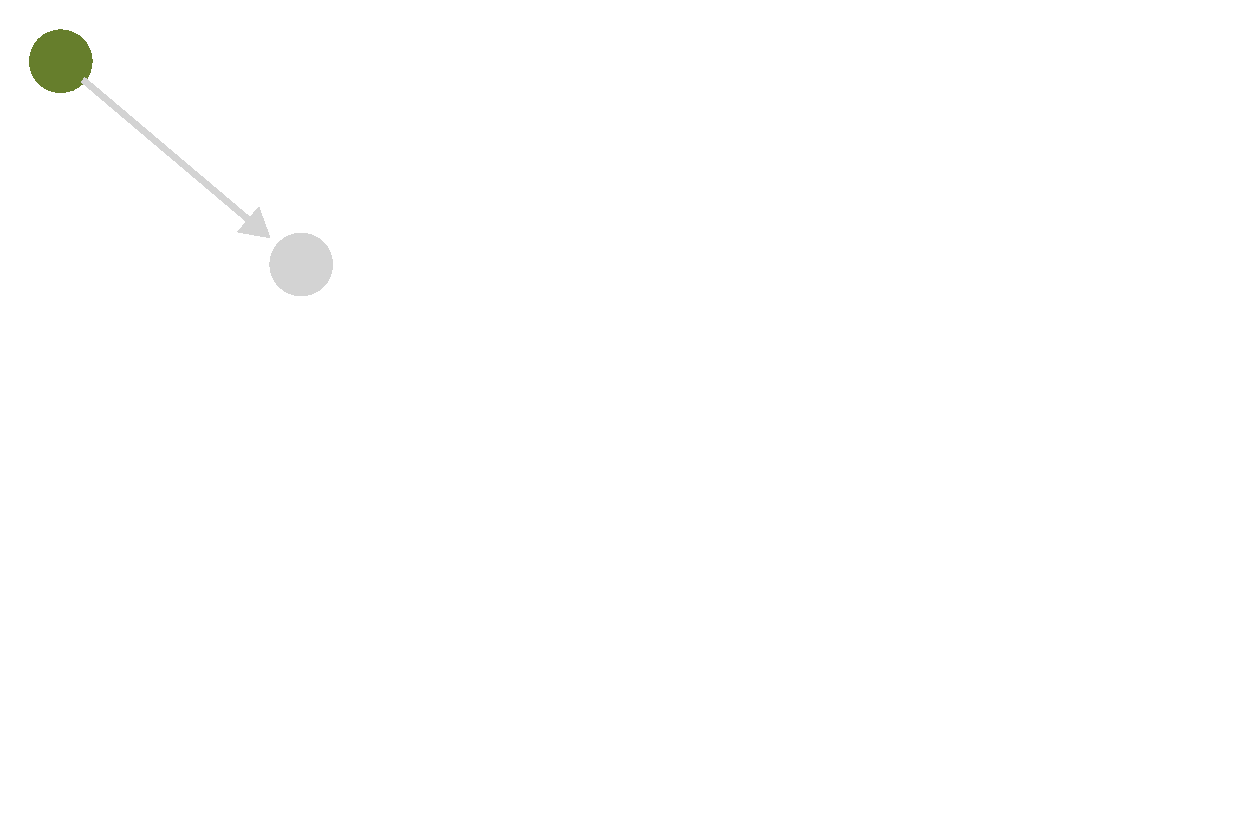
\includegraphics[width=\linewidth]{images/showing-link-traversal-step-0.pdf} % replace with your image file
        \end{column}

        % Right column: Text
        \begin{column}{0.4\textwidth} % Adjust width as needed
            \begin{itemize}
                \item Link Traversal starts from seed documents (URIs)
                \item These are provided by the user or specified in the query
            \end{itemize}
        \end{column}
    \end{columns}
\end{frame}

\begin{frame}{Link Traversal: Traversal}
    \begin{columns}[T] % T aligns columns at the top
        % Left column: Image
        \begin{column}{0.6\textwidth} % Adjust width as needed
            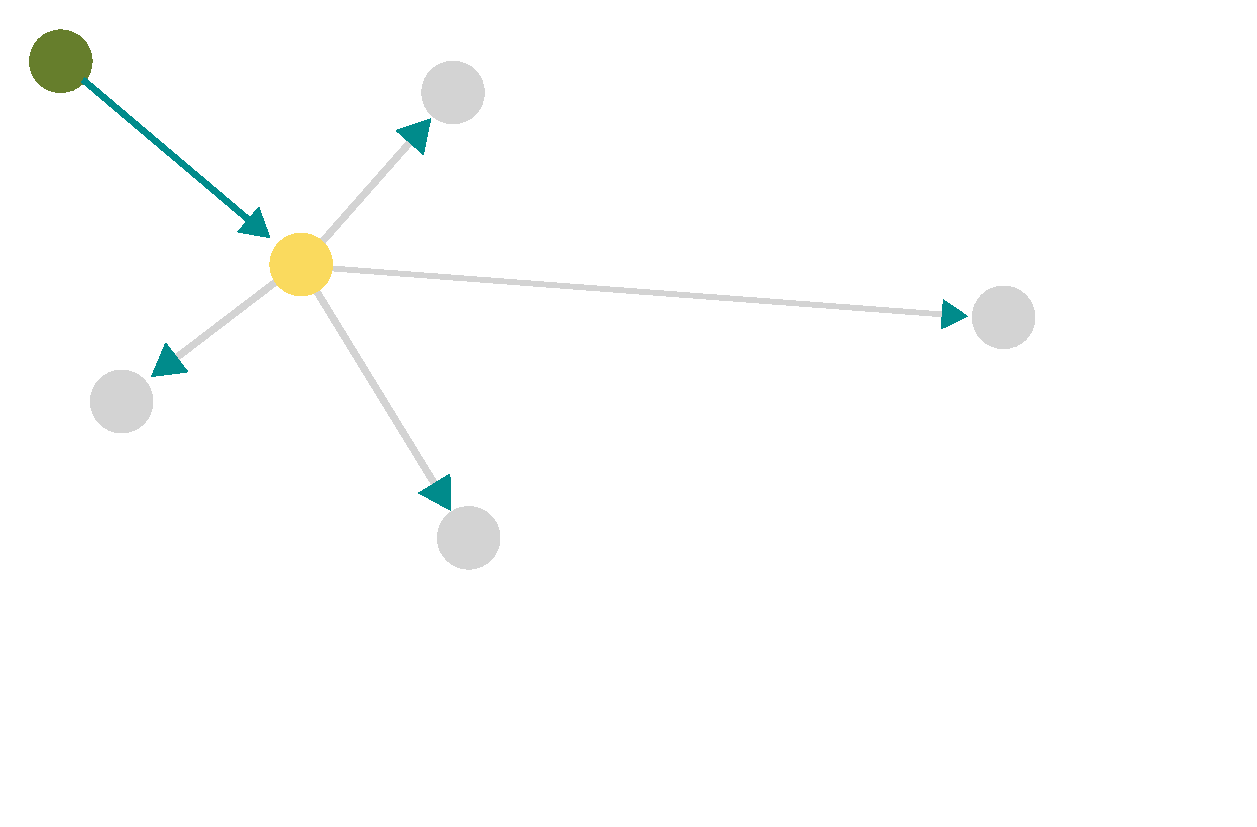
\includegraphics[width=\linewidth]{images/showing-link-traversal-step-1.pdf} % replace with your image file
        \end{column}

        % Right column: Text
        \begin{column}{0.4\textwidth} % Adjust width as needed
            \begin{itemize}
                \item New URIs are extracted from the seed document
                \item URIs are extracted in accordance with reachability criteria
                \item Uses the follow-your-nose principle
            \end{itemize}
        \end{column}
    \end{columns}
\end{frame}


\begin{frame}{Link Traversal: Traversal}
    \begin{columns}[T] % T aligns columns at the top
        % Left column: Image
        \begin{column}{0.6\textwidth} % Adjust width as needed
            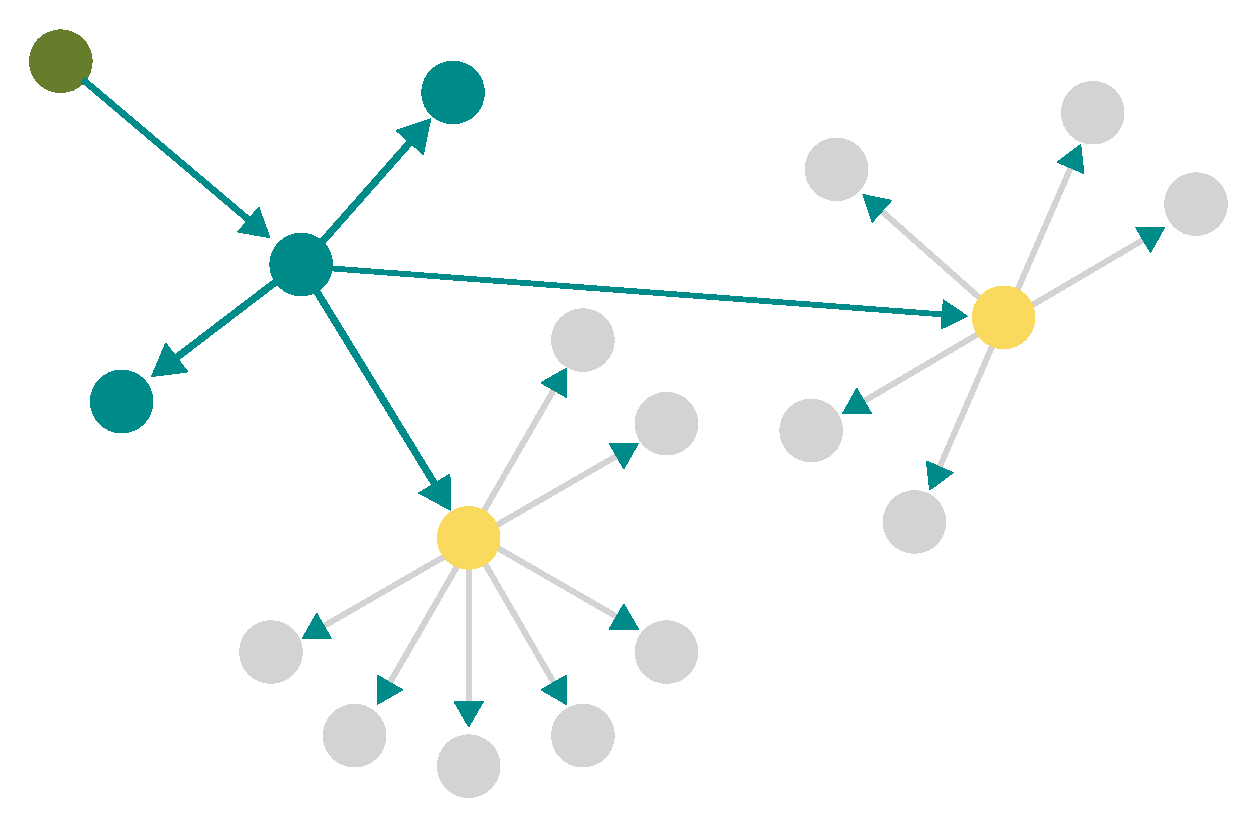
\includegraphics[width=\linewidth]{images/showing-link-traversal-step-2.pdf} % replace with your image file
        \end{column}

        % Right column: Text
        \begin{column}{0.4\textwidth} % Adjust width as needed
            \begin{itemize}
                \item New URIs are dereferenced and the process is repeated
            \end{itemize}
        \end{column}
    \end{columns}
\end{frame}



\begin{frame}{Link Traversal: Termination}
    \begin{columns}[T] % T aligns columns at the top
        % Left column: Image
        \begin{column}{0.6\textwidth} % Adjust width as needed
            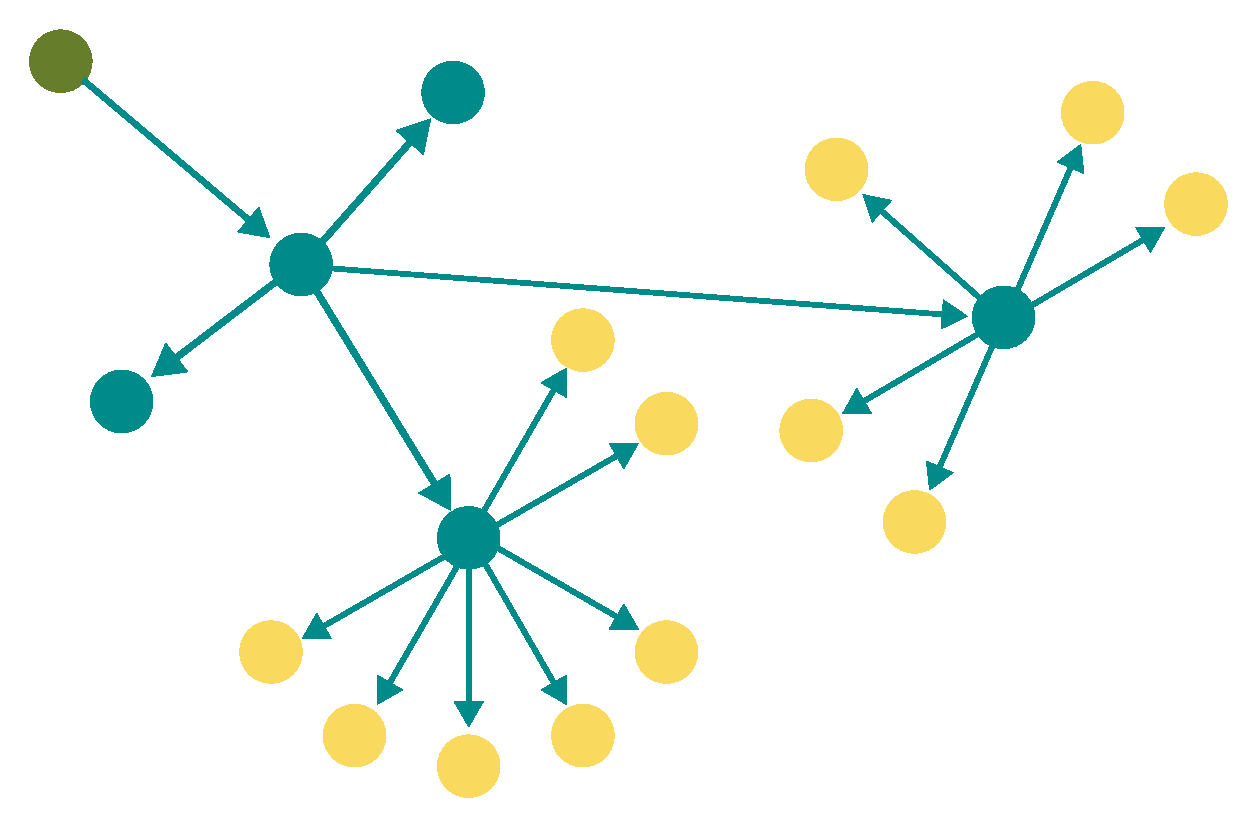
\includegraphics[width=\linewidth]{images/showing-link-traversal-step-3.pdf} % replace with your image file
        \end{column}

        % Right column: Text
        \begin{column}{0.4\textwidth} % Adjust width as needed
            \begin{itemize}
                \item This continues until all links are dereferenced
                \item Continuously produces results
            \end{itemize}
        \end{column}
    \end{columns}
\end{frame}
% NOTES (DONE):
%    - Show how planning ties in with traversal, explain how we assume optimize-then-execute paradigm so plan is fixed (DONE)
%    - Fix link queue image, arrow is the wrong way
% while traversal isn't.

\begin{frame}{Query Optimization for Link Traversal}
    \begin{columns}[T] % T aligns columns at the top
        % Left column: Image
        \begin{column}{0.6\textwidth} % Adjust width as needed
            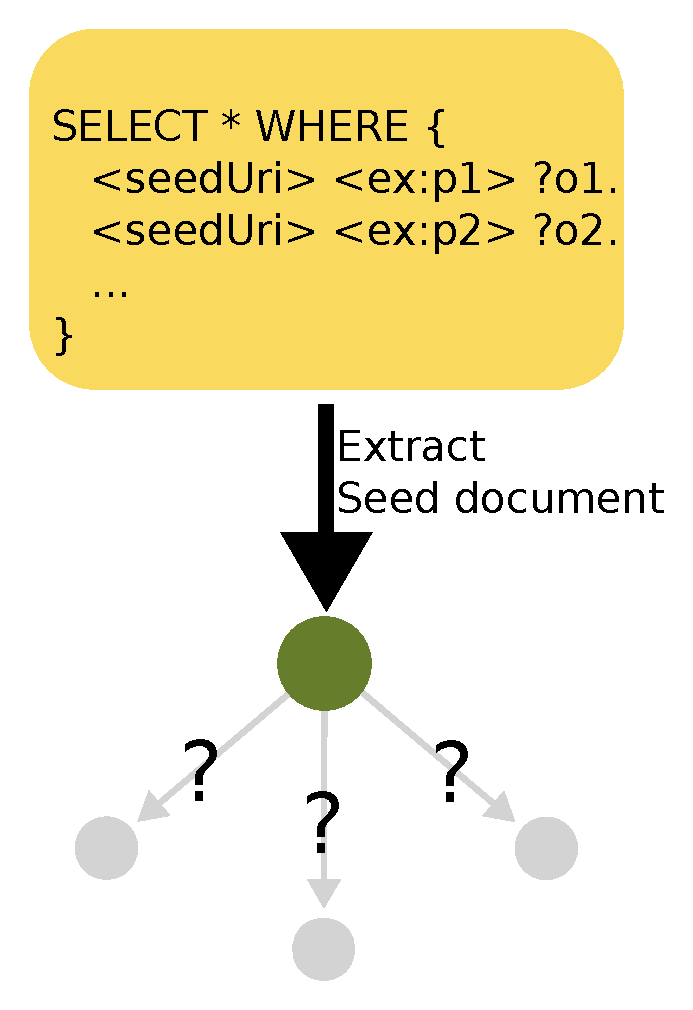
\includegraphics[width=.60\linewidth]{images/hardToOptimizeLTQP.pdf} % replace with your image file
        \end{column}

        % Right column: Text
        \begin{column}{0.4\textwidth}
            The query (partly) determines:
            \begin{itemize}
                \item The queried data
                \item The topology of the queried data
                \item The query-relevant documents
            \end{itemize}
            Result: Limited prior knowledge for query optimization
        \end{column}
    \end{columns}
\end{frame}

\begin{frame}{Query Optimization for Link Traversal: Client-side Engines}
    \begin{columns}[T] % T aligns columns at the top
        % Left column: Image
        \begin{column}{0.6\textwidth} % Adjust width as needed
            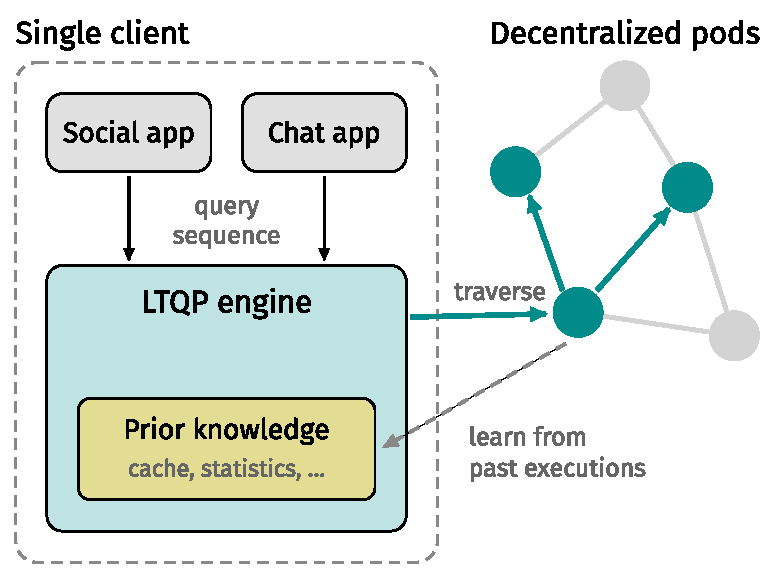
\includegraphics[width=\linewidth]{images/client-side-engine.pdf}
        \end{column}

        % Right column: Text
        \begin{column}{0.4\textwidth}
            \begin{itemize}
                \item Engine instances serve a single client
                \item Can we exploit client-specific usage patterns and `personalize' optimization 
                \item Gain prior knowledge by looking at past executions
            \end{itemize}
        \end{column}
    \end{columns}
\end{frame}



\begin{frame}{Problem Statement}
    \centering
    Evaluating the performance of client-specific optimization techniques in realistic, user-specific scenarios
\end{frame}

% NOTES:
%   - Existing approaches answer the "what are the alternatives?" question from the problem statement
%   - Usage patterns motivate what SolidSessionBench simulates (sessions, interests, refinement)

\begin{frame}{Existing Evaluation Approaches}
  \begin{columns}[T]
    \begin{column}{0.6\textwidth}
      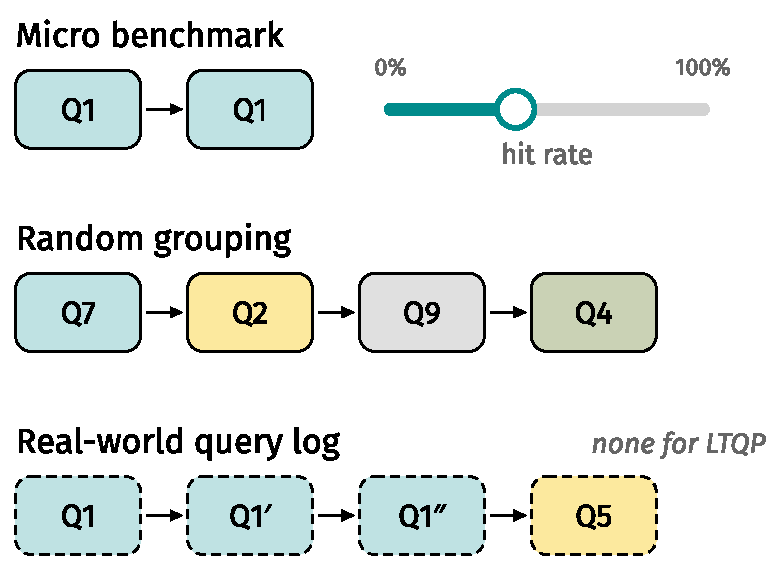
\includegraphics[width=\linewidth]{images/evaluation-approaches.pdf}
    \end{column}

    \begin{column}{0.4\textwidth}
      \begin{itemize}
        \item Micro benchmarks isolate single variables \parencite{hartig2011caching,nicholson2024hpcache}
        \item End-to-end benchmarks group unrelated queries \parencite{bizer2011berlin,martin2010improving}
        \item Real-world query logs are the gold standard \parencite{saleem2015lsq}, but none exist for LTQP
      \end{itemize}
    \end{column}
  \end{columns}
\end{frame}

\begin{frame}{Towards a Shared Simulated Benchmark}
  \begin{itemize}\setlength\itemsep{1em}
    \item Next best option: a unified simulated benchmark
    \item Common basis for comparison and improved reproducibility
    \item Grounded in usage patterns observed in the literature:
      \begin{itemize}
        \item User interest-based query behavior
        \item Logical query sessions
        \item Query refinement
      \end{itemize}
  \end{itemize}
\end{frame}

\begin{frame}{Usage Patterns: User Interest-Based Query Behavior}
  \begin{columns}[T]
    \begin{column}{0.6\textwidth}
      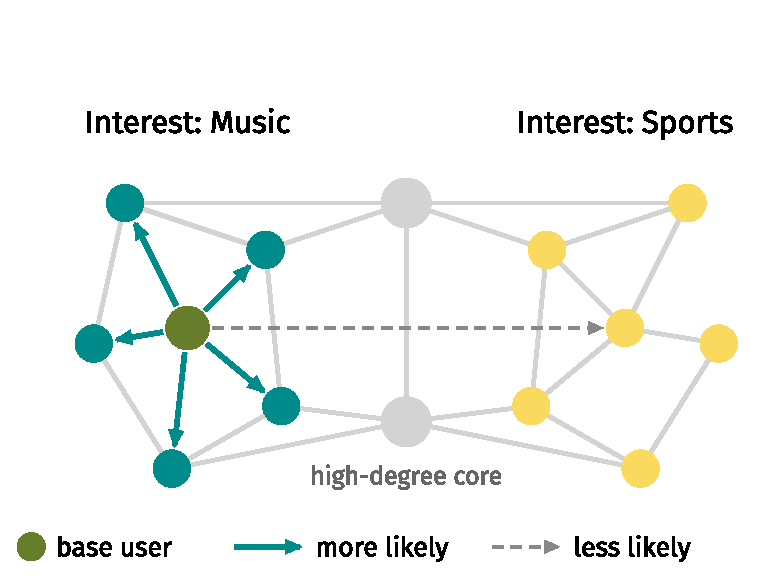
\includegraphics[width=\linewidth]{images/user-interests.pdf}
    \end{column}

    \begin{column}{0.4\textwidth}
      \begin{itemize}
        \item Users form communities based on shared interests \parencite{mislove2007measurement}
        \item Shared interests drive more interactions between users \parencite{mitzlaff2013user}
        \item[$\Rightarrow$] Simulate user-relatedness when choosing what to query
      \end{itemize}
    \end{column}
  \end{columns}
\end{frame}

\begin{frame}{Usage Patterns: Logical Query Sessions}
  \begin{columns}[T]
    \begin{column}{0.6\textwidth}
      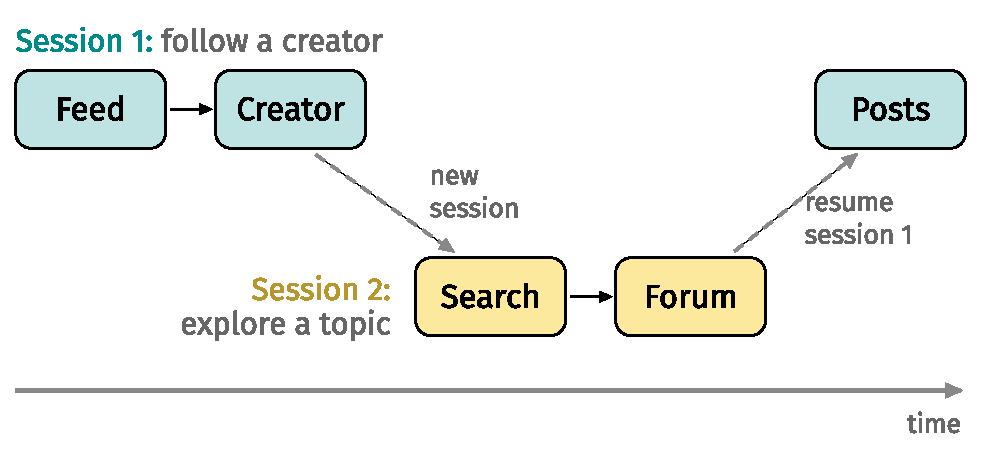
\includegraphics[width=\linewidth]{images/logical-sessions.pdf}
    \end{column}

    \begin{column}{0.4\textwidth}
      \begin{itemize}
        \item Browsing is grouped into goal-oriented logical sessions \parencite{meiss_whats_2009}
        \item New sessions begin in approximately 15\% of clicks
        \item Next query builds on previous results
        \item[$\Rightarrow$] Simulate dependent queries and session switching
      \end{itemize}
    \end{column}
  \end{columns}
\end{frame}

\begin{frame}{Usage Patterns: Query Refinement}
  \begin{columns}[T]
    \begin{column}{0.55\textwidth}
      \begin{block}{SPARQL query logs \parencite{bonifati2020analytical}}
        \begin{itemize}
          \item Related queries are issued in streaks
          \item Iteratively refined towards a shared goal
          \item Mostly adding or removing \texttt{FILTER}, \texttt{UNION}, and \texttt{OPTIONAL}
        \end{itemize}
      \end{block}
    \end{column}
    \begin{column}{0.4\textwidth}
      \begin{block}{Exploratory querying \parencite{arenas2025exploring}}
        \begin{itemize}
          \item Result refinement
          \item Result generalization
          \item Result extension
          \item Bug fixing
          \item Query refinement
          \item Shifting query intent
        \end{itemize}
      \end{block}
    \end{column}
  \end{columns}
  \vspace{1em}
  $\Rightarrow$ Queries evolve step-by-step instead of being independent templates
\end{frame}

\begin{frame}{Usage Patterns: Query Refinement Example}
  \centering
  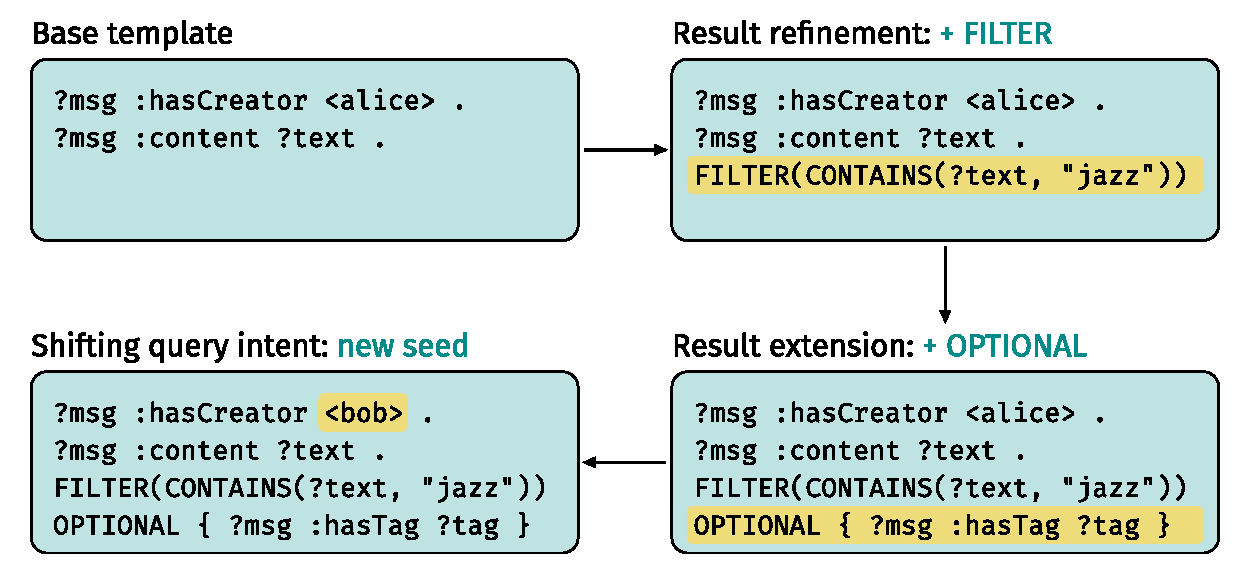
\includegraphics[width=.85\linewidth]{images/query-refinement.pdf}
\end{frame}

\begin{frame}{Simulation Methodology: Base Benchmark}
  \begin{block}{Simulated Solid Environment: SolidBench \parencite{taelman2023link}}
    \begin{itemize}
        \item Based on the realistic LDBC Social Network Benchmark
        \item Data is stored in vaults simulating social media application
    \end{itemize}
  \end{block}
  \begin{block}{Data attributes}
        \begin{itemize}
            \item Generates 158,233~RDF files 
            \item Across 1,531~data vaults
            \item containing a total of 3,556,159~triples.
    \end{itemize}
  \end{block}
\end{frame}

% \begin{frame}[t]{Metrics Used}
%     \begin{itemize}
%         \item Time until first result and last result
%         \item Relative to breadth-first traversal baseline
%         \item $R^{3}$
%     \end{itemize}
% \end{frame}

% NOTES:
%   - Each usage pattern from the literature maps to one step of the generator
%   - Figures are illustrative, similarity/probability values are made up (softmax is computed correctly for T = 0.1)

\begin{frame}{Simulation Methodology: Extending SolidBench}
    \centering
    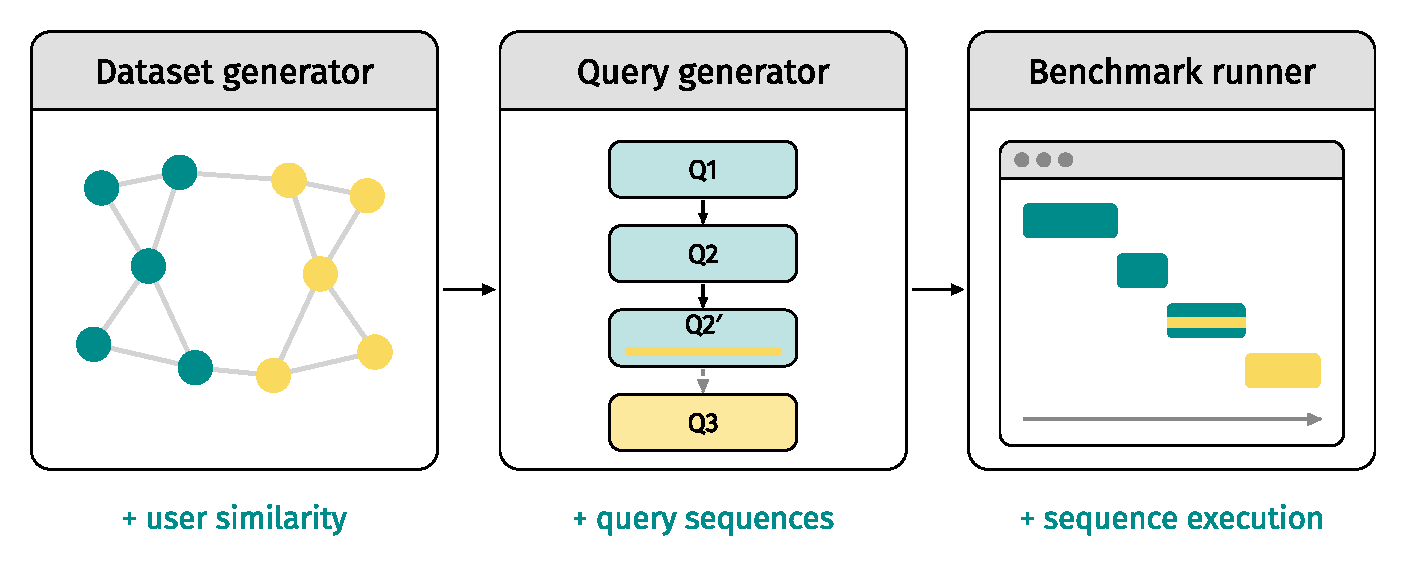
\includegraphics[width=\linewidth]{images/solidbench-extensions.pdf}
\end{frame}

\begin{frame}{Simulation Methodology: Generating a Query Sequence}
    \centering
    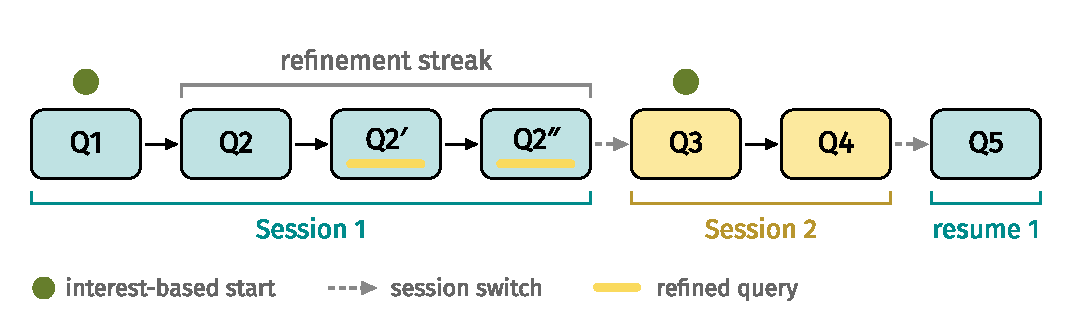
\includegraphics[width=.85\linewidth]{images/sequence-overview.pdf}

    \vspace{0.5em}
    \raggedright
    \begin{itemize}
        \item Each sequence starts from a randomly selected base user
        \item Sessions chain dependent queries, refinement streaks modify them step-by-step
        \item A single seeded random generator keeps sequences reproducible
    \end{itemize}
\end{frame}


\begin{frame}{Usage Pattern: Logical Sessions}
    \begin{columns}[c]
        \begin{column}{0.5\textwidth}
            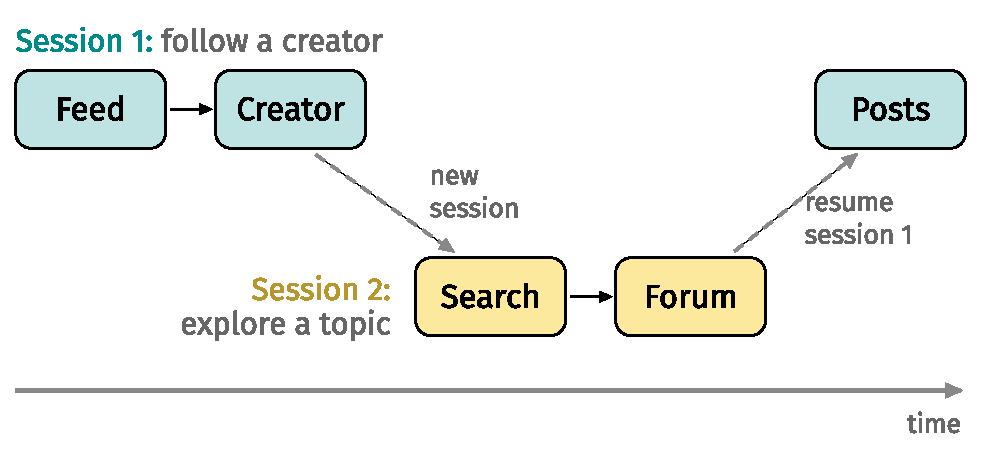
\includegraphics[width=\linewidth]{images/logical-sessions.pdf}
        \end{column}

        \begin{column}{0.5\textwidth}
            \small
            \begin{block}{Observed \parencite{meiss_whats_2009}}
                \begin{itemize}
                    \item Browsing groups into goal-oriented sessions
                    \item New sessions in $\sim$15\% of clicks
                \end{itemize}
            \end{block}
            \begin{block}{Simulated}
                \begin{itemize}
                    \item Next query instantiated from previous results
                    \item Switch to a new session or resume an old one
                \end{itemize}
            \end{block}
        \end{column}
    \end{columns}
\end{frame} 

\begin{frame}{Usage Pattern: User Interests}
    \begin{columns}[T]
        \begin{column}{0.5\textwidth}
            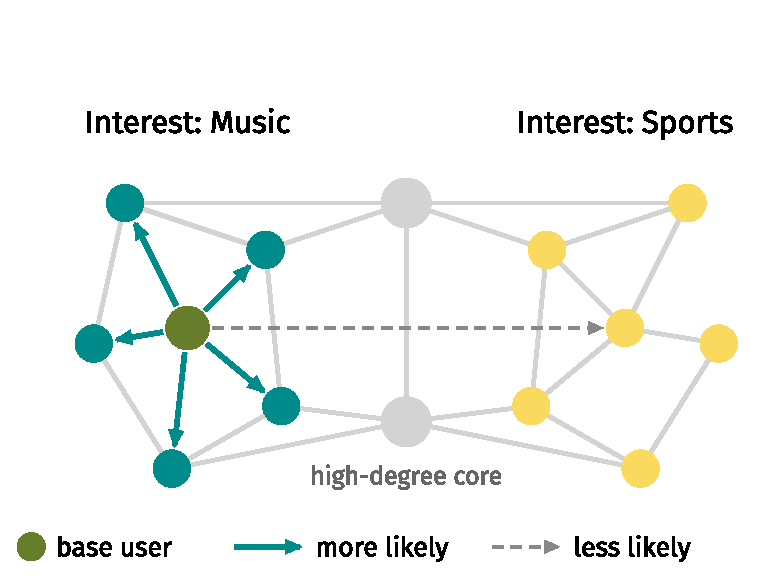
\includegraphics[width=\linewidth]{images/user-interests.pdf}
        \end{column}

        \begin{column}{0.5\textwidth}
            \small
            \begin{block}{Observed \parencite{mislove2007measurement,mitzlaff2013user}}
                \begin{itemize}
                    \item Users form communities around shared interests
                    \item Shared interests drive more interactions
                \end{itemize}
            \end{block}
            \begin{block}{Simulated}
                \begin{itemize}
                    \item User similarity on interests and studies
                    \item Similar users are more likely to start a session
                \end{itemize}
            \end{block}
        \end{column}
    \end{columns}
\end{frame}


\begin{frame}{Usage Pattern: Query Refinement}
    \centering
    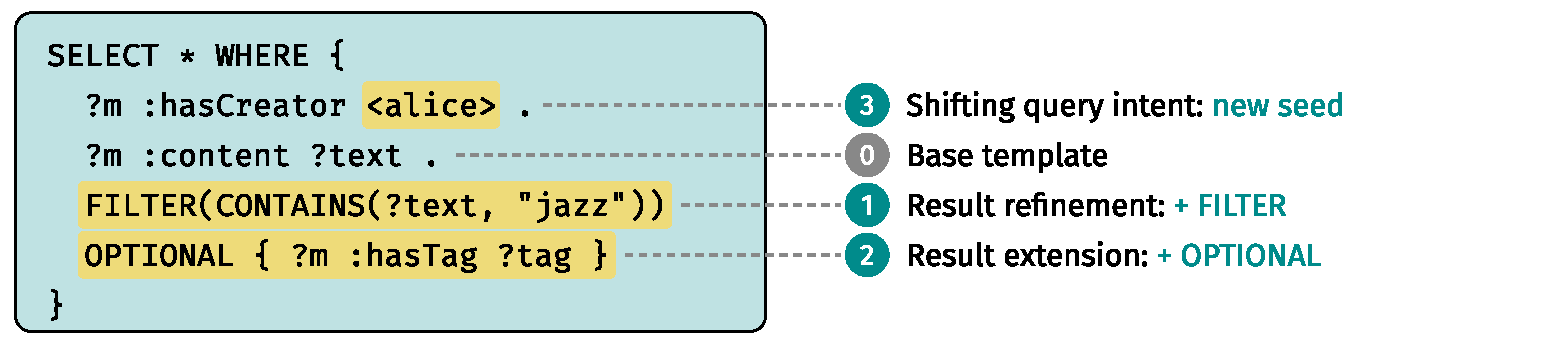
\includegraphics[width=\linewidth]{images/query-refinement-wide.pdf}

    \begin{columns}[T]
        \begin{column}{0.48\textwidth}
            \small
            \begin{block}{Observed \parencite{bonifati2020analytical,arenas2025exploring}}
                \begin{itemize}
                    \item Queries refined step-by-step
                    \item Mostly \texttt{FILTER}, \texttt{UNION}, \texttt{OPTIONAL}
                \end{itemize}
            \end{block}
        \end{column}
        \begin{column}{0.48\textwidth}
            \small
            \begin{block}{Simulated}
                \begin{itemize}
                    \item Composable transformations on queries
                    \item Randomly select sequence of transformations to add to query sequence
                \end{itemize}
            \end{block}
        \end{column}
    \end{columns}
\end{frame}

% NOTES:
%   - Caching is the simplest client-side optimization that exploits past queries
%   - If sequences are realistic, cache hit rates should reflect sessions and refinement
%   - Goal is benchmark validation, not an exhaustive cache comparison

\begin{frame}{Validating the Benchmark: Client-side Caching}
    \begin{itemize}\setlength\itemsep{1em}
        \item Caching directly exploits data from past queries \parencite{hartig2011caching}
        \item Correlated query sequences should lead to cache hits
        \item Cache hit rates reveal whether our sequences behave as intended
        \item[$\Rightarrow$] Goal: validate the benchmark, not an exhaustive cache comparison
    \end{itemize}
\end{frame}

\begin{frame}{Caching Approaches}
    \centering
    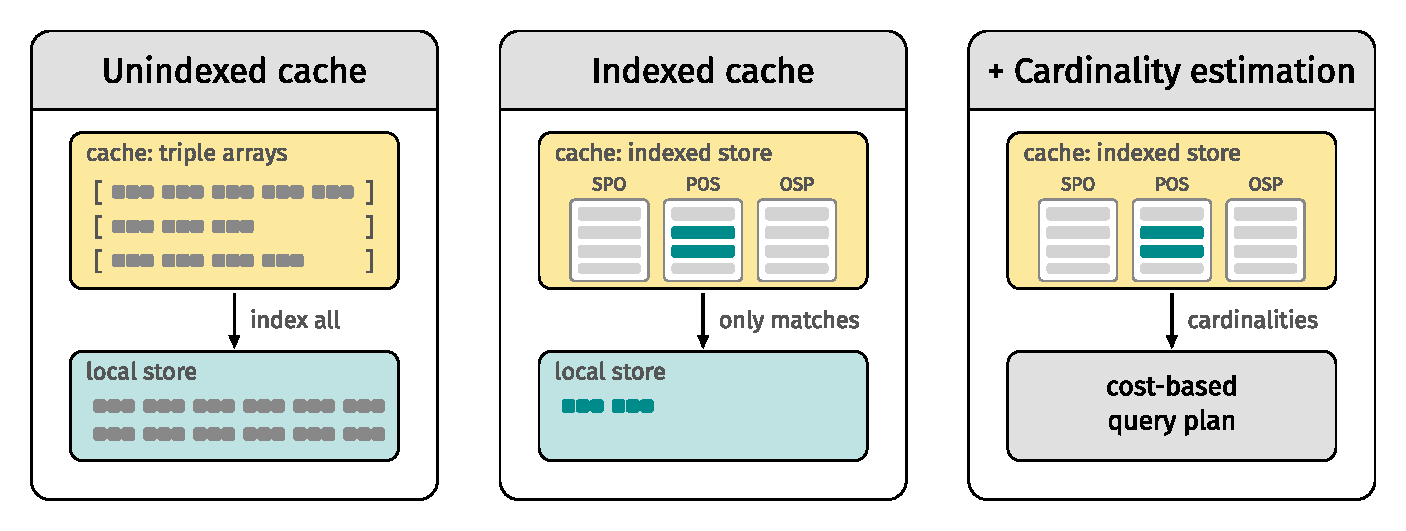
\includegraphics[width=\linewidth]{images/cache-approaches.pdf}

    \vspace{0.5em}
    Implemented in Comunica \parencite{taelman2018comunica}, LRU eviction, three sizes: S (350k quads, $\sim$10\%), M (700k, $\sim$20\%), L (1.4M, $\sim$40\%)
\end{frame}

\begin{frame}{Experimental Setup}
  \begin{block}{Workload}
    \begin{itemize}
        \item 8 generated sequences, 192 queries (discover and short templates)
    \end{itemize}
  \end{block}
  \begin{block}{Execution}
    \begin{itemize}
        \item Each sequence repeated 10 times, 70--90 ms injected network latency, 180 s timeout
        \item Cache scoped to a single sequence, no state shared between runs
    \end{itemize}
  \end{block}
  \begin{block}{Measured}
    \begin{itemize}
        \item Cache hit rates, evictions, and speedup over no cache
    \end{itemize}
  \end{block}
\end{frame}

% NOTES:
%   - Core message: realistic sequences expose session and refinement effects,
%     other evaluation methods miss them or point to the wrong conclusion
%   - Session chart is drawn from Table 2 of the paper (mean over all 9 cache configurations)

\begin{frame}{Results: All Caches Outperform No Caching}
    \centering
    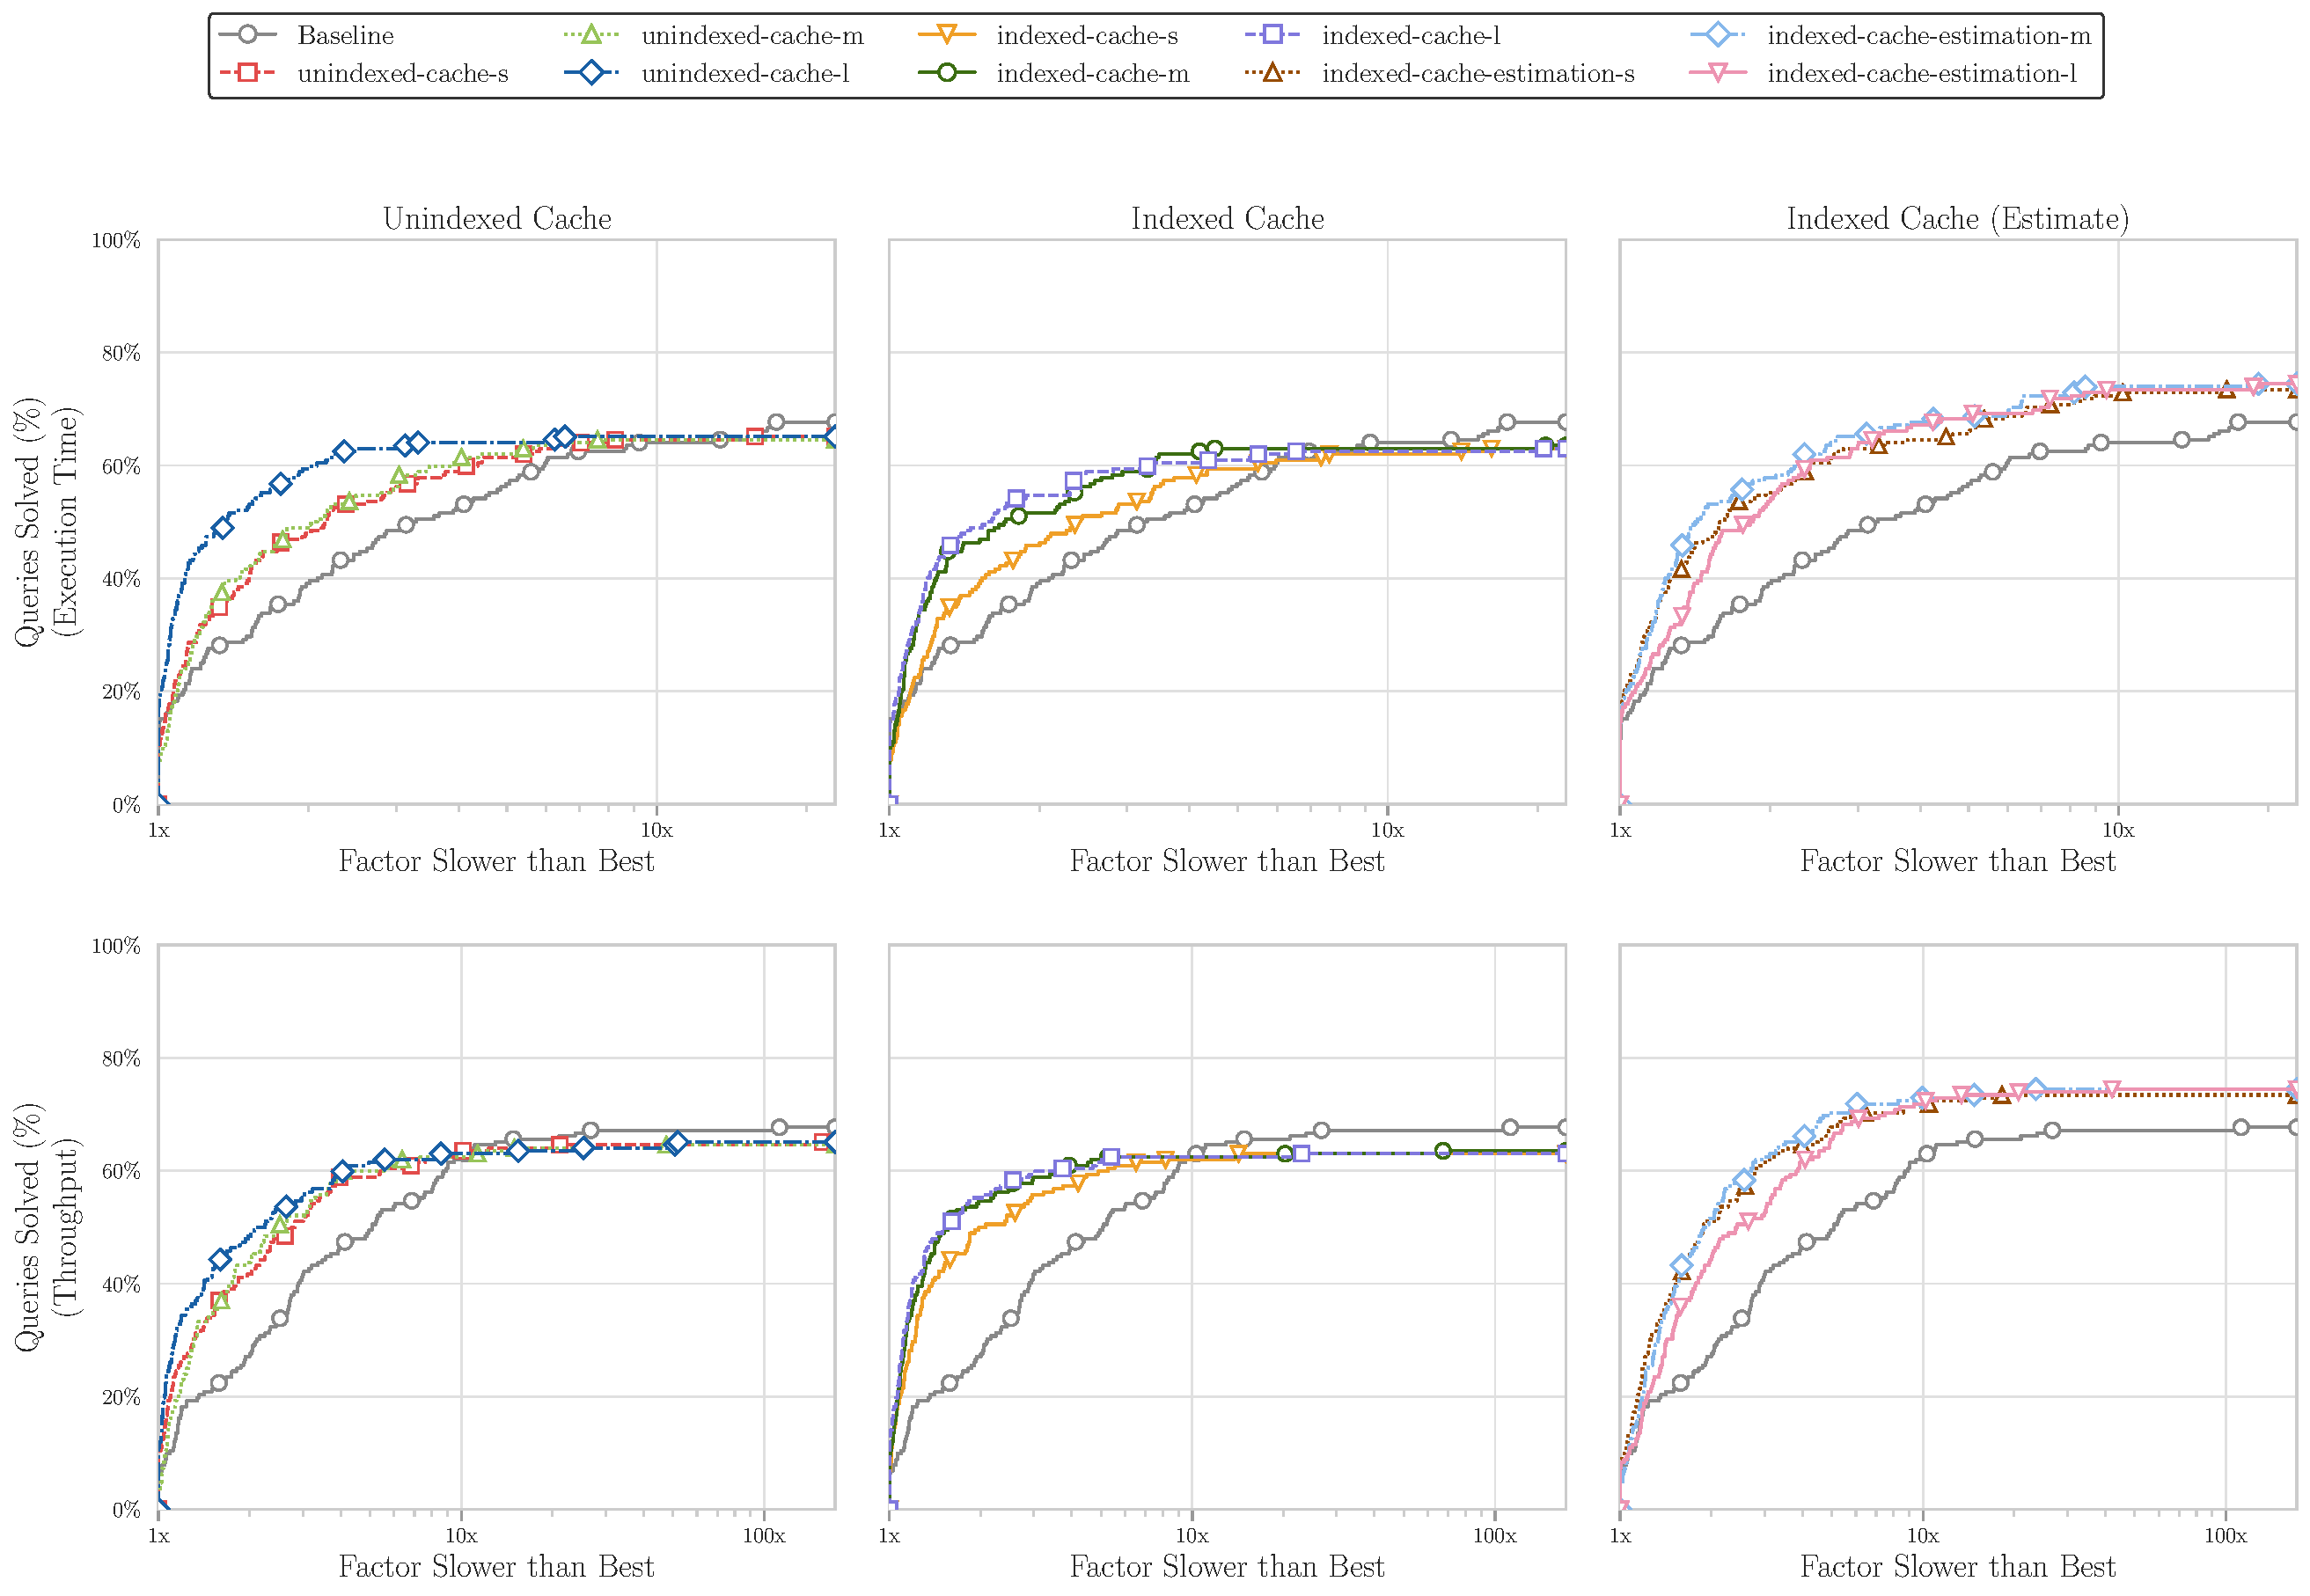
\includegraphics[width=.88\linewidth,trim=0 393 0 0,clip]{images/performance_profile.pdf}

    \footnotesize
    Performance profile \parencite{dolan2002benchmarking}: higher and further left is better
    \normalsize

    \vspace{0.5em}
    Cardinality estimation performs best and solves the most queries
\end{frame}

\begin{frame}{Results: Session Switching Costs Cache Hits}
    \begin{columns}[T]
        \begin{column}{0.55\textwidth}
            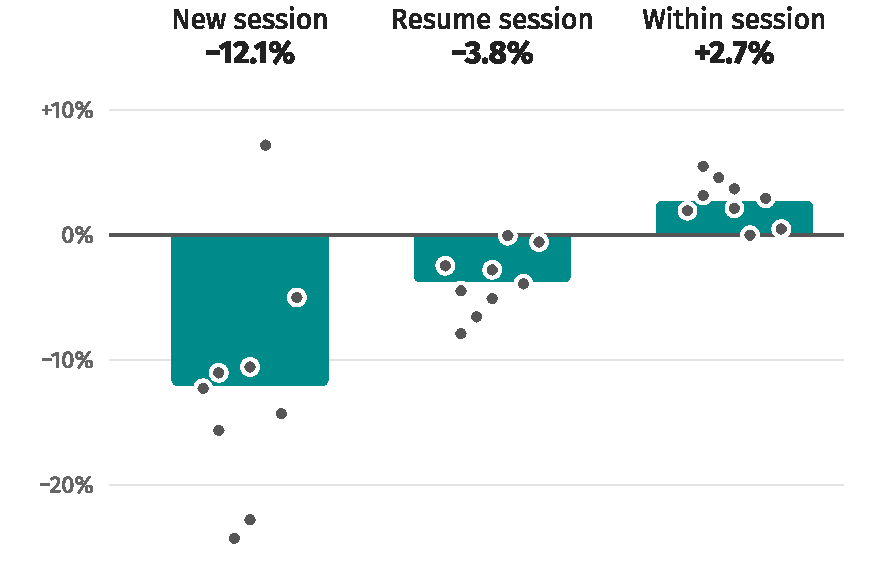
\includegraphics[width=\linewidth]{images/session-hit-rates.pdf}
        \end{column}

        \begin{column}{0.45\textwidth}
            \begin{itemize}
                \item Hit rate compared to the average of the same template
                \item New sessions: $-12\%$
                \item Staying in a session: $+3\%$
                \item[$\Rightarrow$] Cache sizing and eviction depend on session behavior
            \end{itemize}
        \end{column}
    \end{columns}
\end{frame}

\begin{frame}{Results: Refinement Reuses Prior Data}
    \centering
    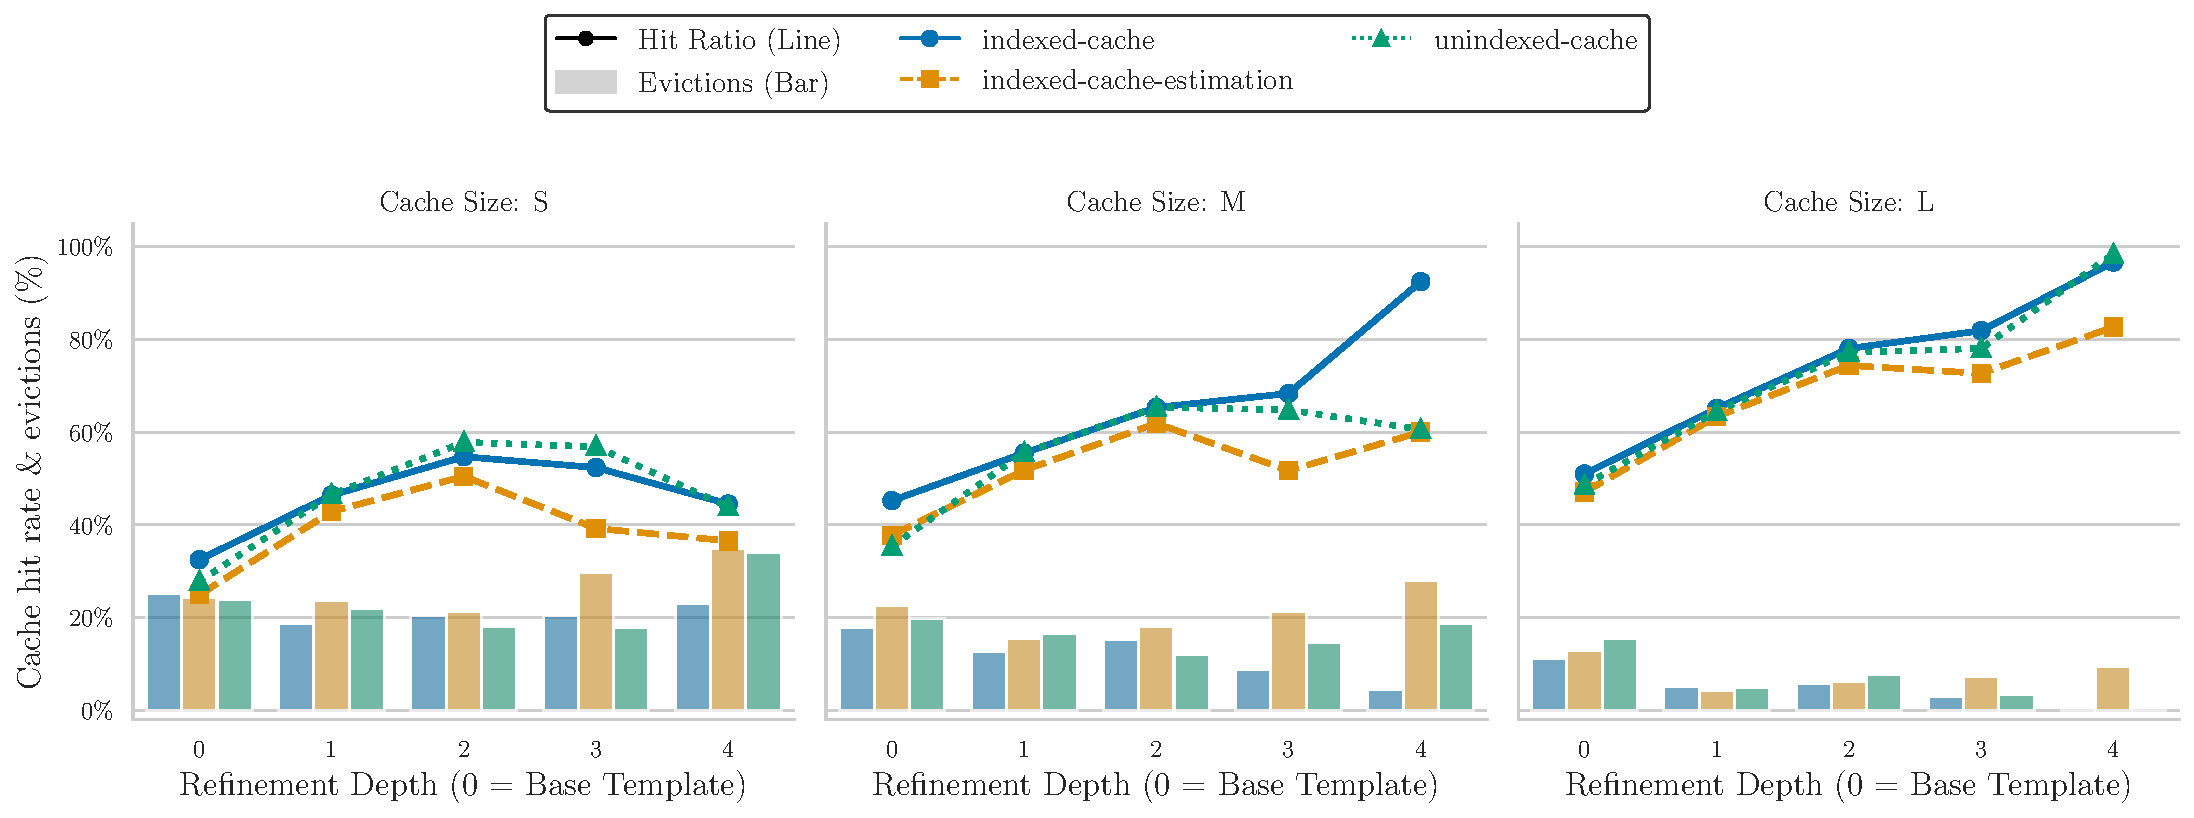
\includegraphics[width=\linewidth]{images/combined_cache_efficiency.pdf}

    \vspace{0.5em}
    Hit rates rise with each refinement step, until small caches start thrashing
\end{frame}

\begin{frame}{Results: Refinement Translates into Speedups}
    \centering
    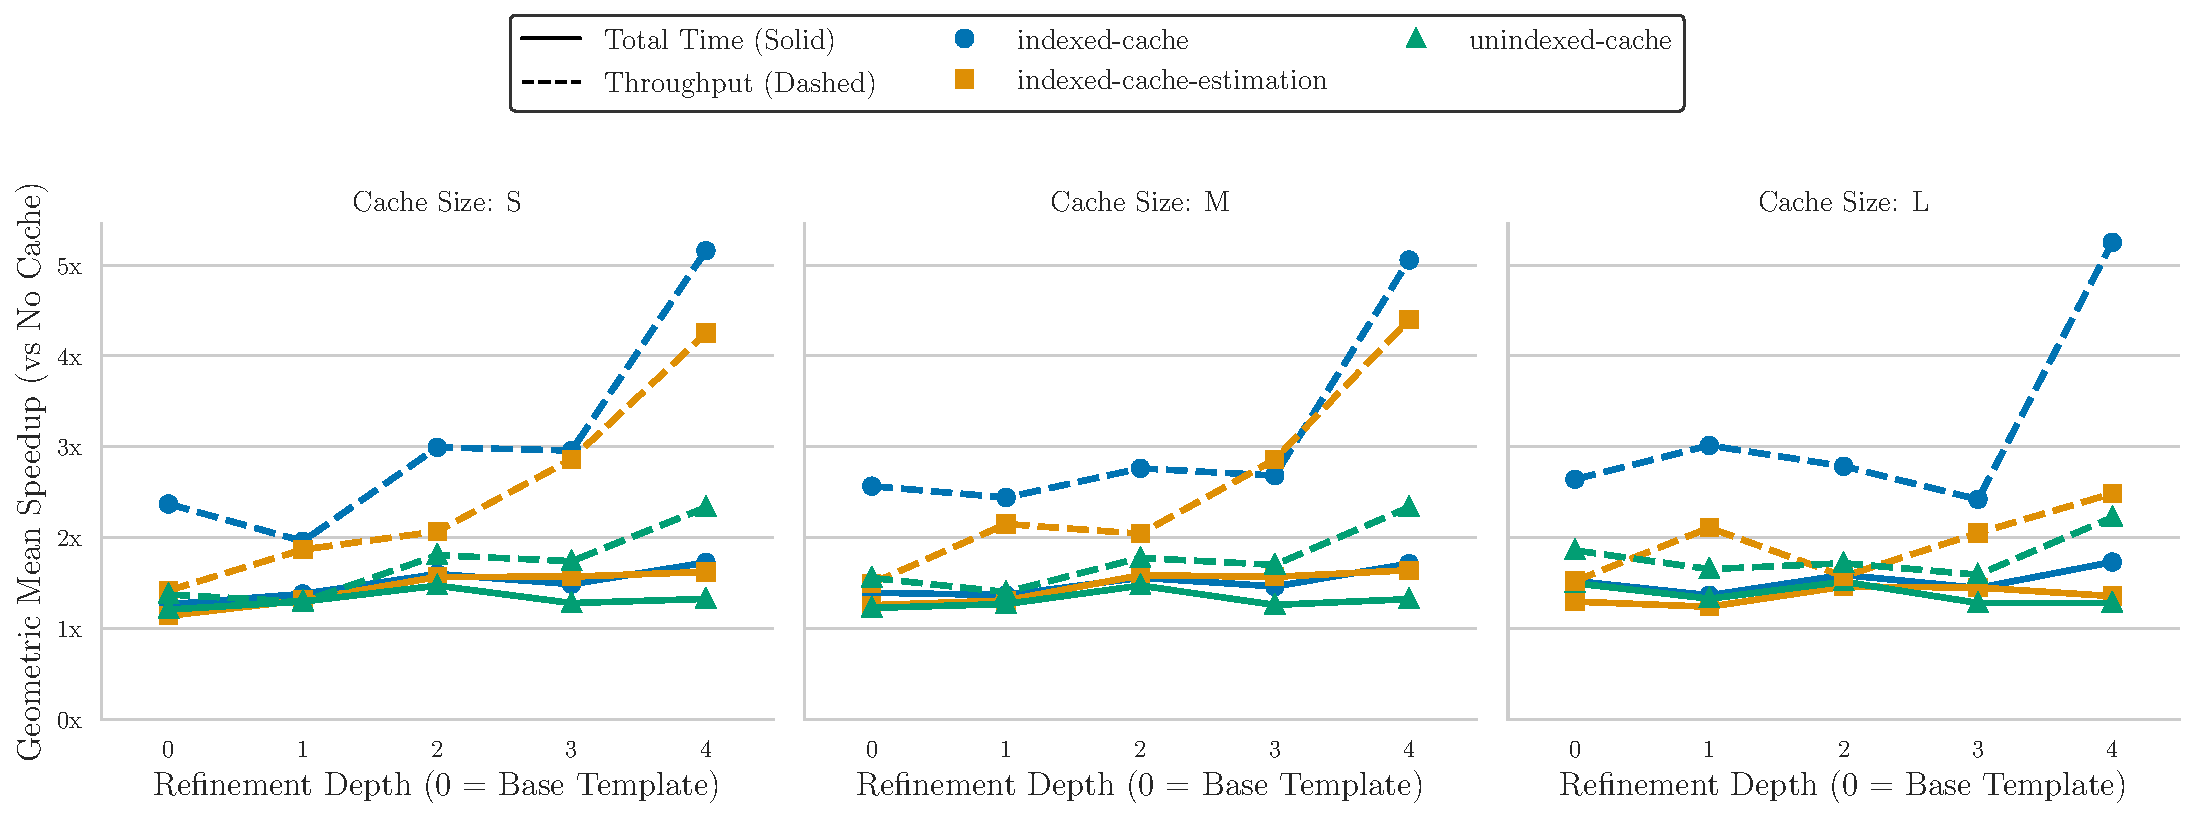
\includegraphics[width=\linewidth]{images/temporal_throughput_line.pdf}

    \vspace{0.5em}
    Up to $\sim$5$\times$ throughput at refinement depth 4 with the indexed cache
\end{frame}

\begin{frame}{Comparison: Random Sequences Mislead}
    % Paper legends cropped off; random panel scaled so both plot areas have the same height
    \begin{columns}[T]
        \begin{column}{0.5\textwidth}
            \centering
            \textbf{Random sequences}

            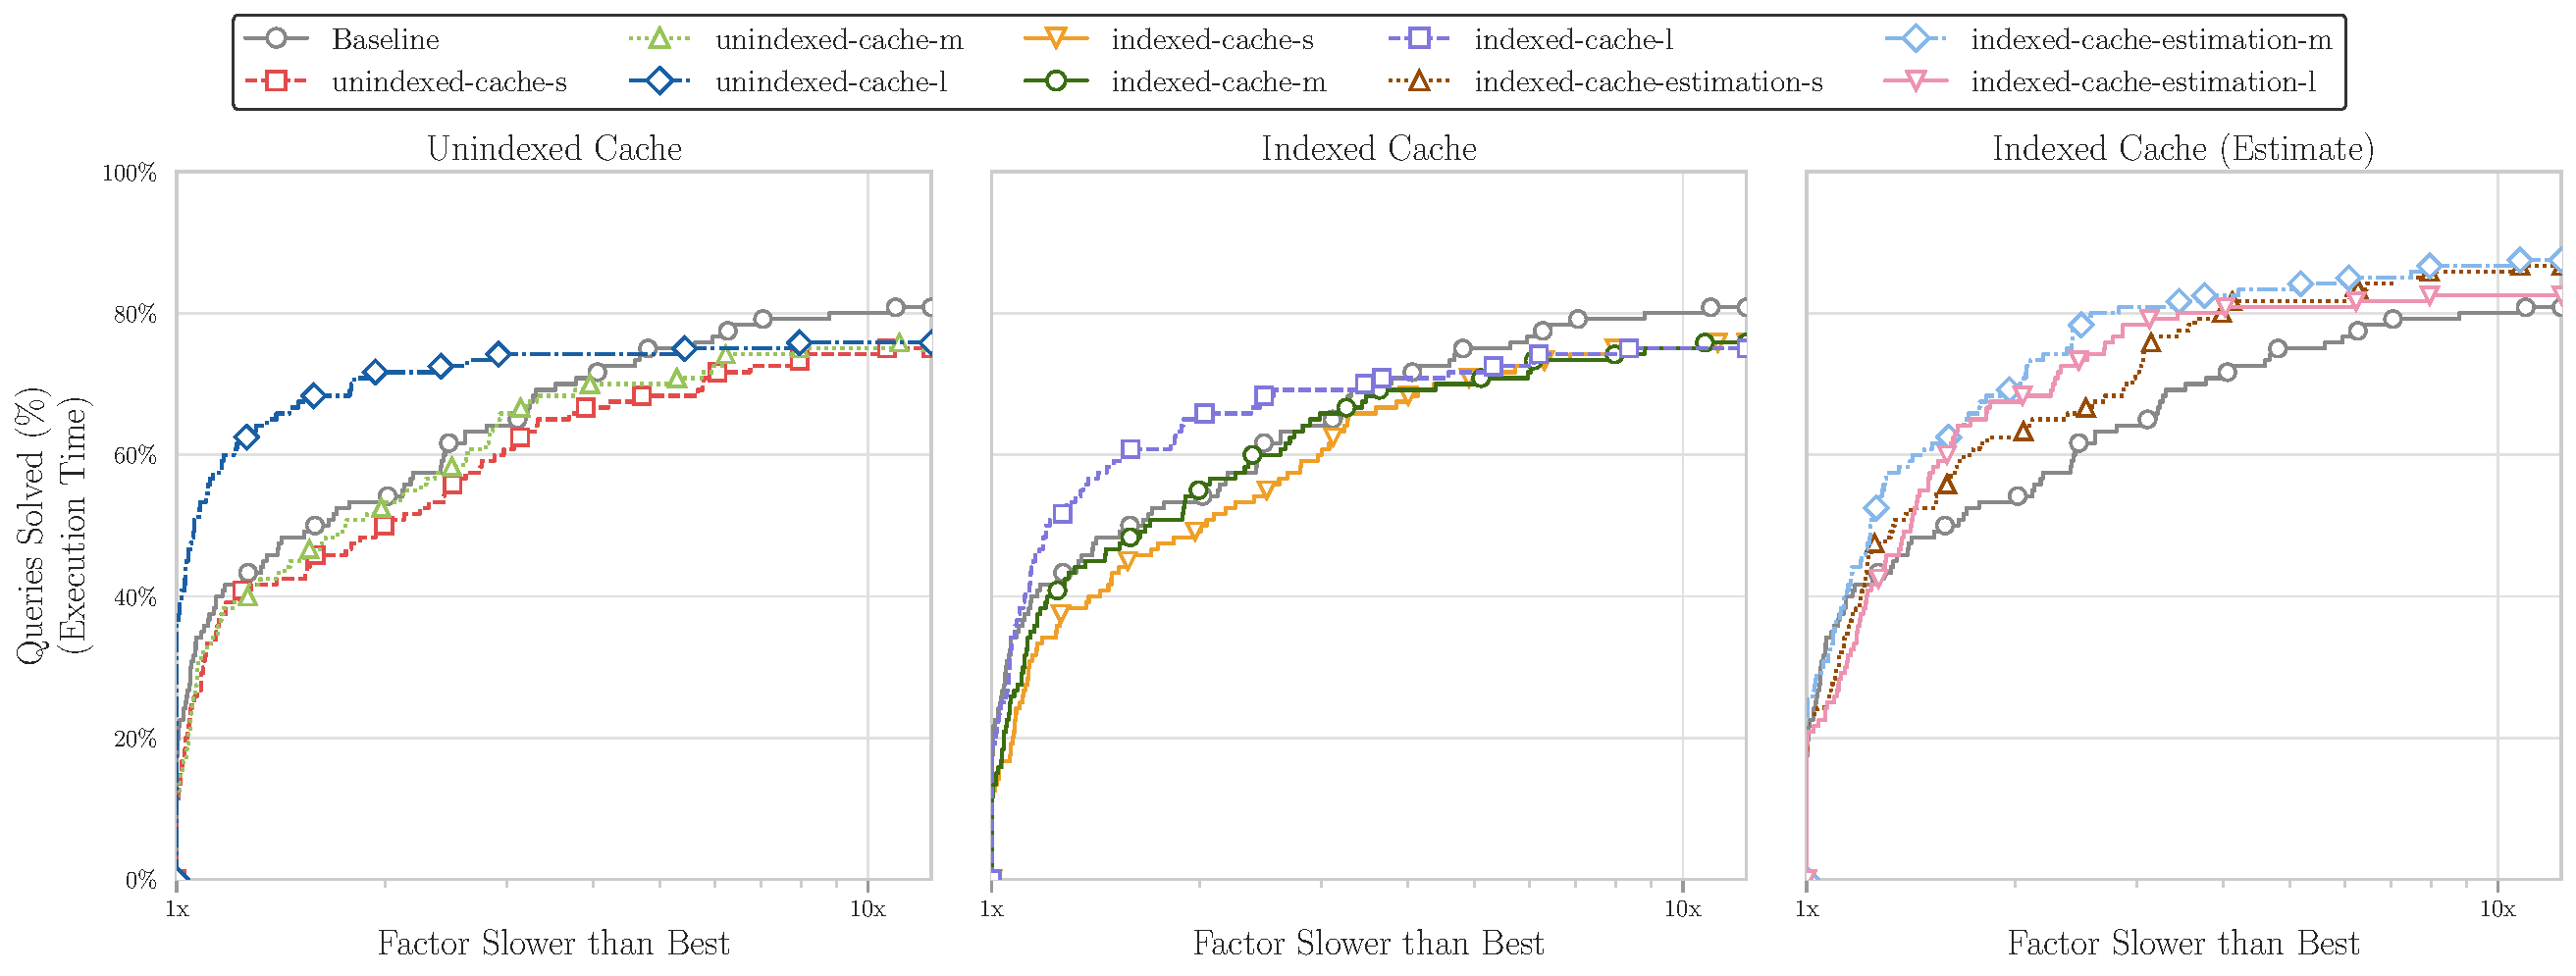
\includegraphics[width=.72\linewidth,trim=0 0 803 80,clip]{images/performance_profile_random_sequences.pdf}
        \end{column}

        \begin{column}{0.5\textwidth}
            \centering
            \textbf{SolidSessionBench}

            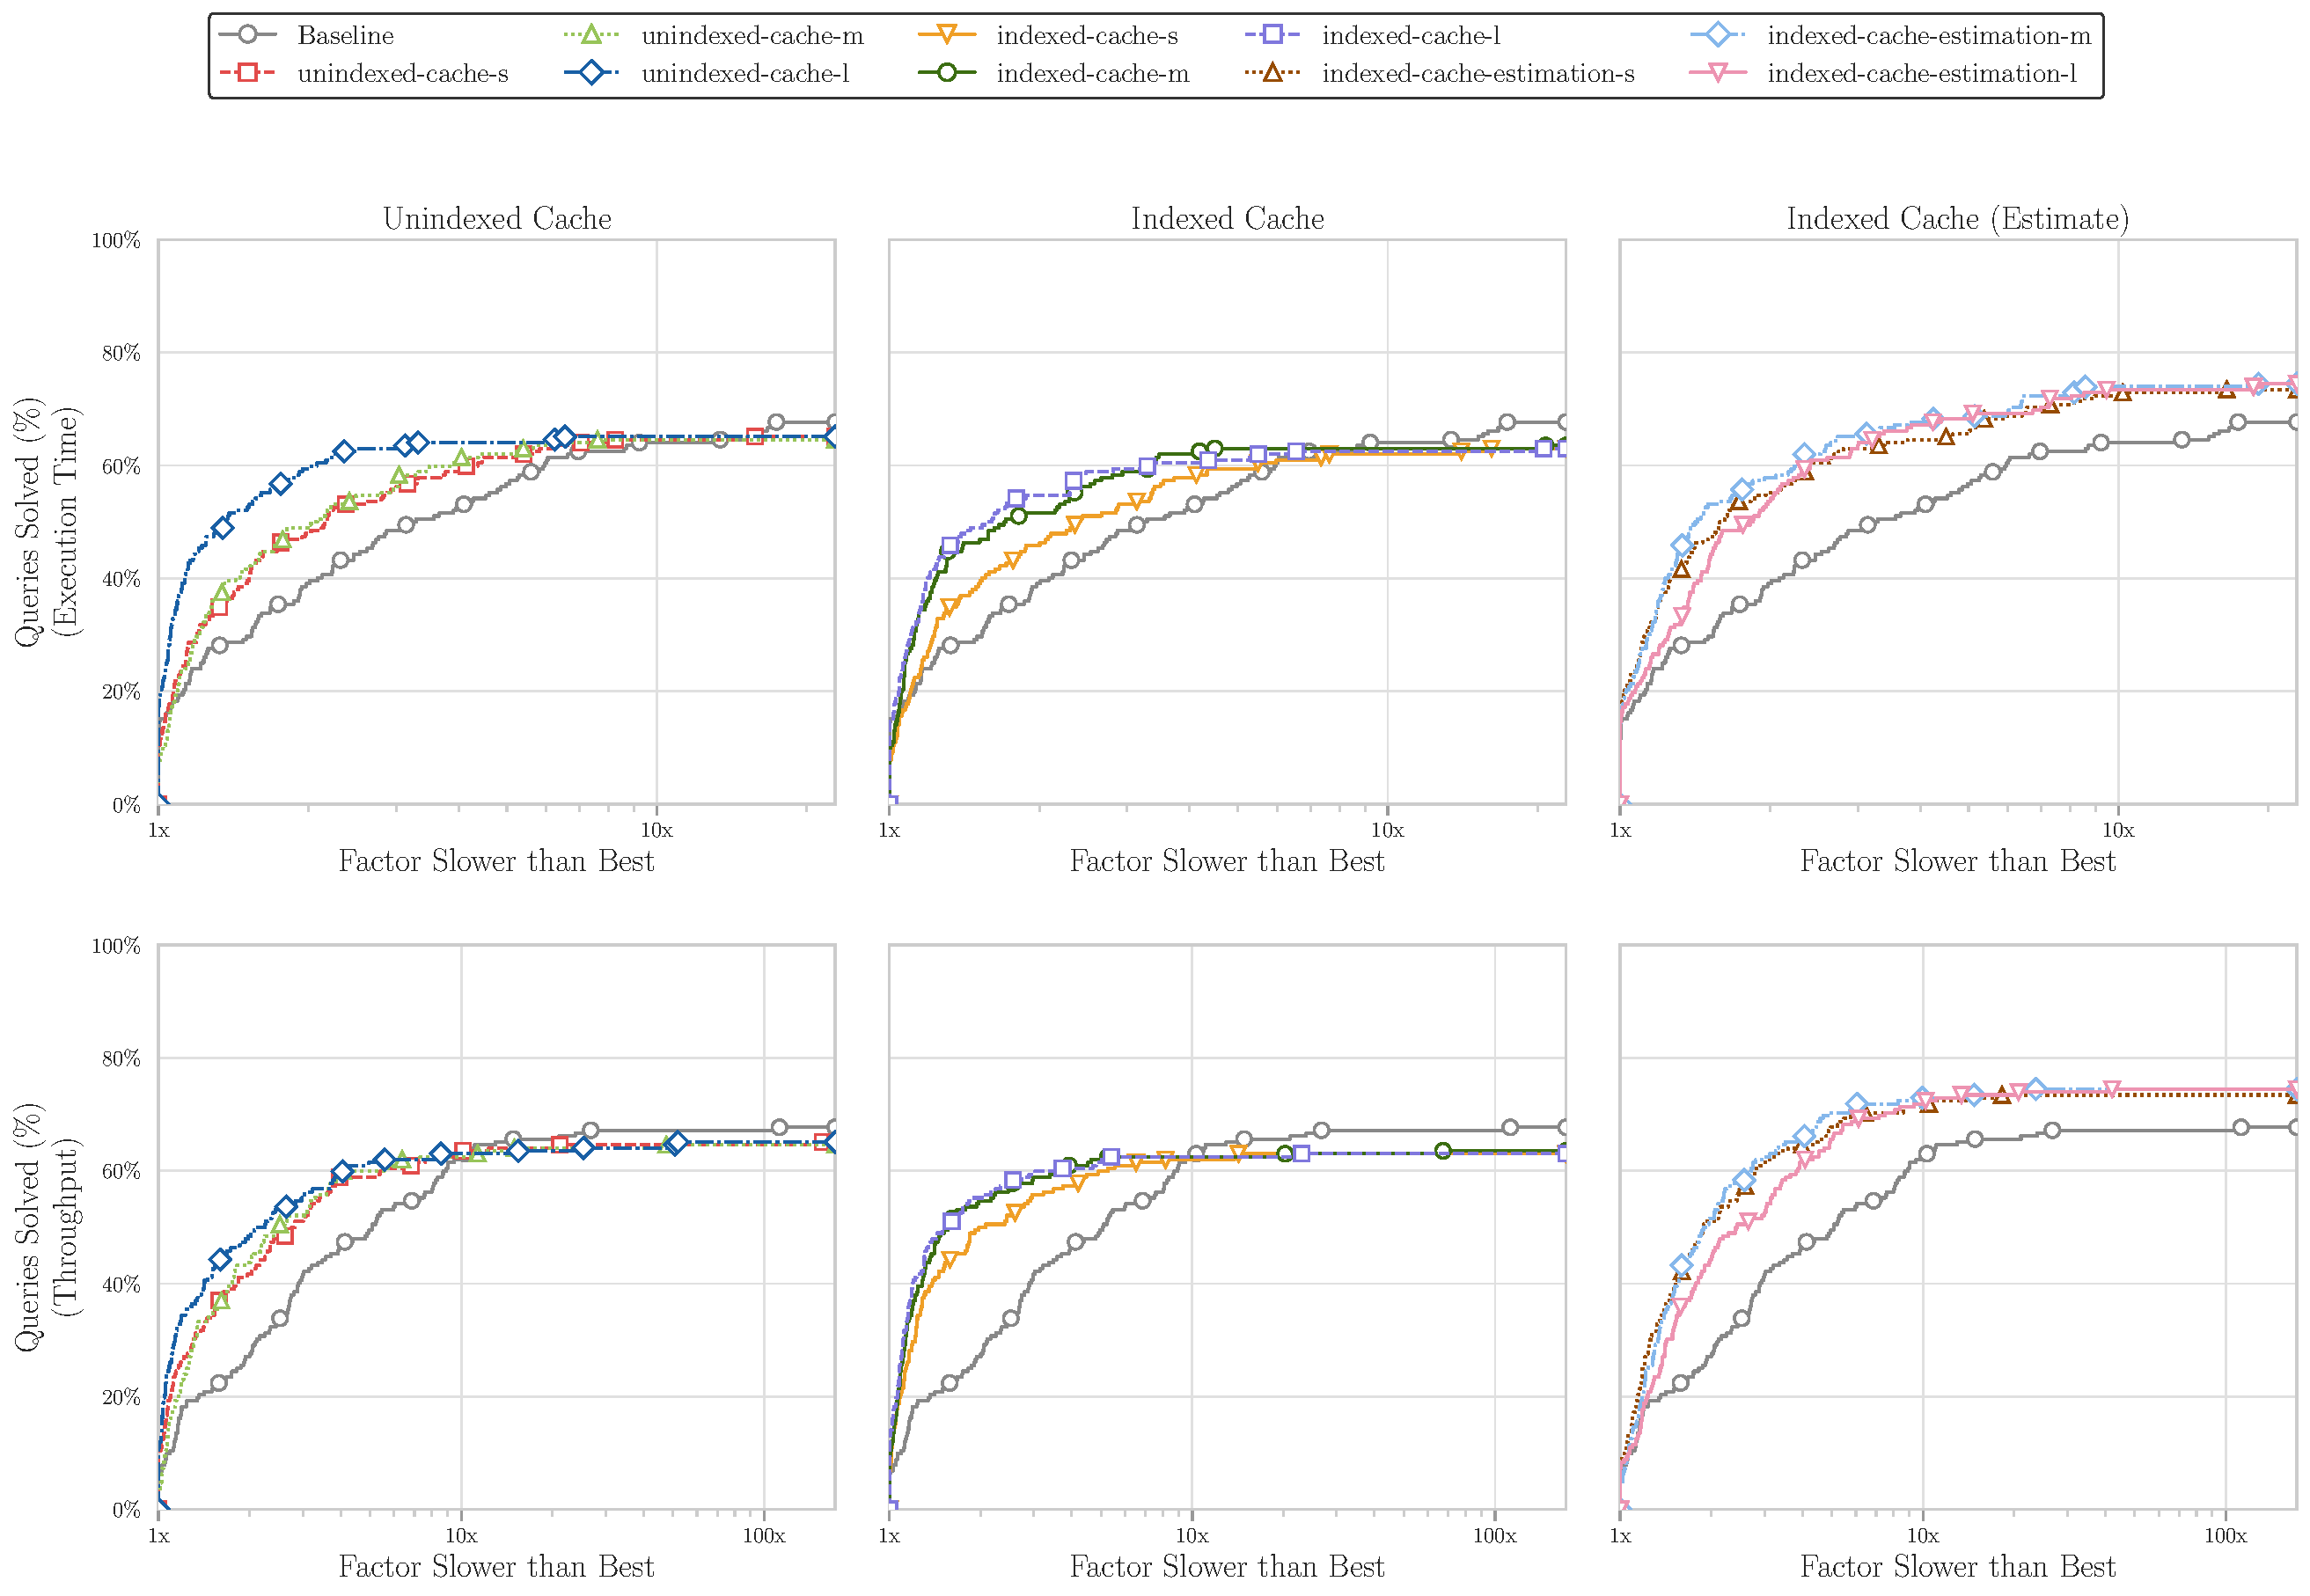
\includegraphics[width=.81\linewidth,trim=0 390 803 125,clip]{images/performance_profile.pdf}
        \end{column}
    \end{columns}

    \vspace{0.3em}
    \centering
    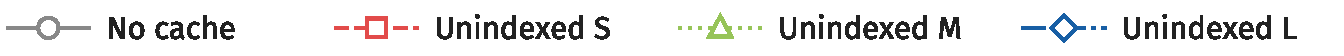
\includegraphics[width=.7\linewidth]{images/legend-unindexed.pdf}

    \vspace{0.5em}
    Random: only large caches help \quad vs.\ \quad SolidSessionBench: small caches help too
\end{frame}

\begin{frame}{Comparison: Micro Benchmarks Give Mixed Signals}
    \begin{columns}[T]
        \begin{column}{0.6\textwidth}
            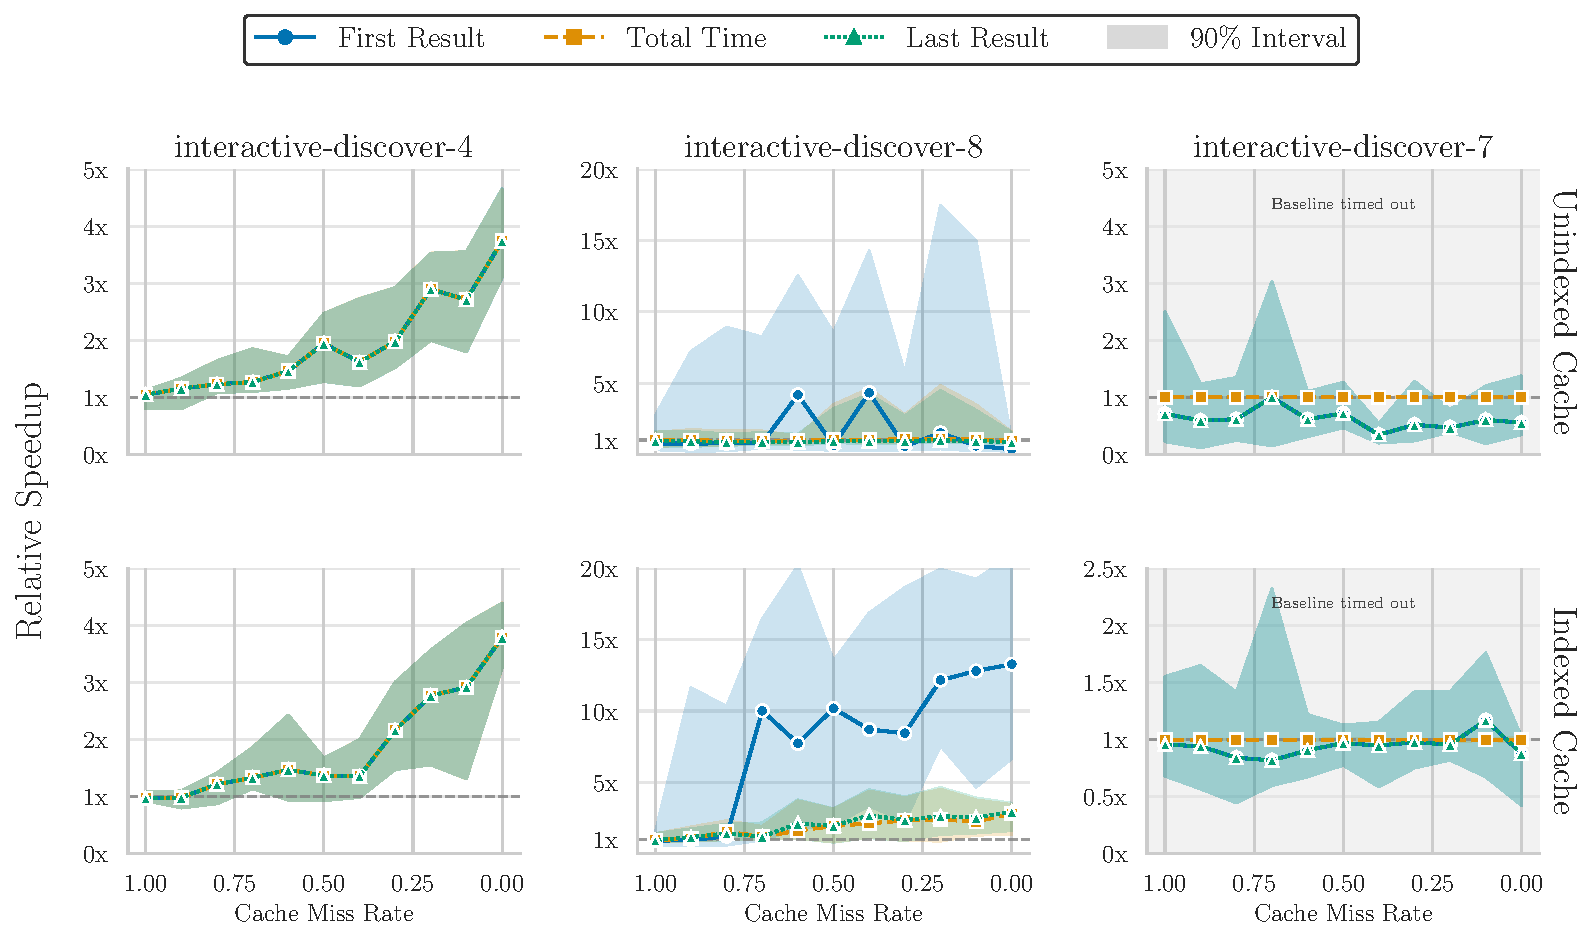
\includegraphics[width=\linewidth]{images/synth_hit_rate_reduced.pdf}
        \end{column}

        \begin{column}{0.4\textwidth}
            \begin{itemize}
                \item Each template run twice with simulated cache miss rates
                \item 8 of 12 templates speed up with hit rate
                \item Long-running queries: no speedup, or even slowdowns
                \item[$\Rightarrow$] Isolated queries do not show behavior in realistic sequences
            \end{itemize}
        \end{column}
    \end{columns}
\end{frame}

\begin{frame}{Key Takeaways}
    \begin{itemize}\setlength\itemsep{1.5em}
        \item Realistic sequences reveal how sessions and refinement drive client-side performance
        \item Random sequences and micro benchmarks miss these effects, or lead to the wrong conclusions
        \item[$\Rightarrow$] SolidSessionBench: a reproducible basis for evaluating client-side optimizations
    \end{itemize}
\end{frame}


% --- Bibliography slide ---
\begin{frame}[allowframebreaks]{References}
  \printbibliography[heading=none]
\end{frame}

\begin{frame}{Simulation Methodology: Hyperparameters}
    \centering
    \begin{tabular}{llr}
        \toprule
        \textbf{Category} & \textbf{Parameter} & \textbf{Value} \\
        \midrule
        Log-normal $(\mu, \sigma)$ & Sequence length          & 3.0, 0.2 \\
                                   & Session length           & 1.7, 0.5 \\
                                   & Transition probability   & $-2.0$, 0.25 \\
        \midrule
        Refinements   & \texttt{patternProbability}       & 0.1 \\
                      & \texttt{min/maxRefinementLength}  & 2, [3--5] \\
        \midrule
        Instantiation & \texttt{temperature}              & 0.1 \\
                      & \texttt{maxLogits}                & 5--10 \\
        \bottomrule
    \end{tabular}

    \vspace{1em}
    A single seeded PRNG guarantees reproducible sequences
\end{frame}

% Detail slides moved out of the main talk; the main talk has one slide per usage pattern

\begin{frame}{Simulation Methodology: Logical Query Sessions}
    \begin{columns}[T]
        \begin{column}{0.6\textwidth}
            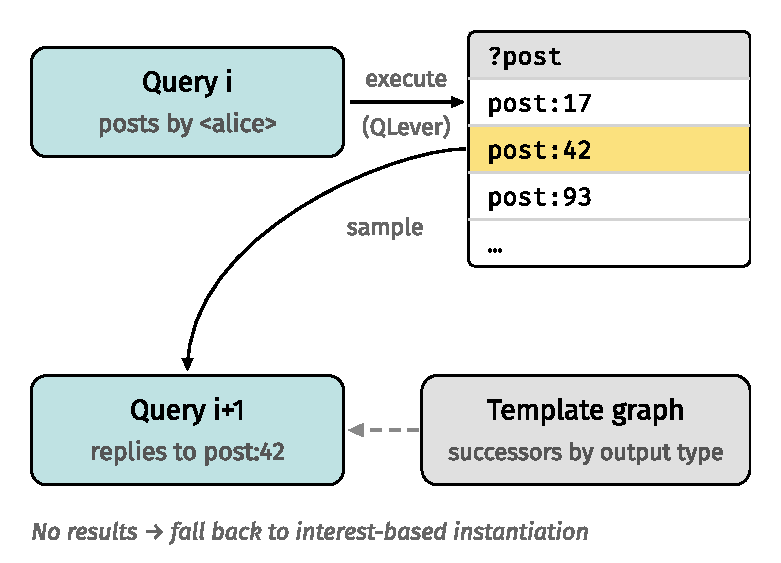
\includegraphics[width=\linewidth]{images/click-through-instantiation.pdf}
        \end{column}

        \begin{column}{0.4\textwidth}
            \begin{itemize}
                \item Directed template graph: output types map to valid next templates
                \item Instantiation values sampled from previous results
                \item Simulates ``click-through'' behavior
            \end{itemize}
        \end{column}
    \end{columns}
\end{frame}

\begin{frame}{Simulation Methodology: Session Switching}
    \begin{columns}[T]
        \begin{column}{0.6\textwidth}
            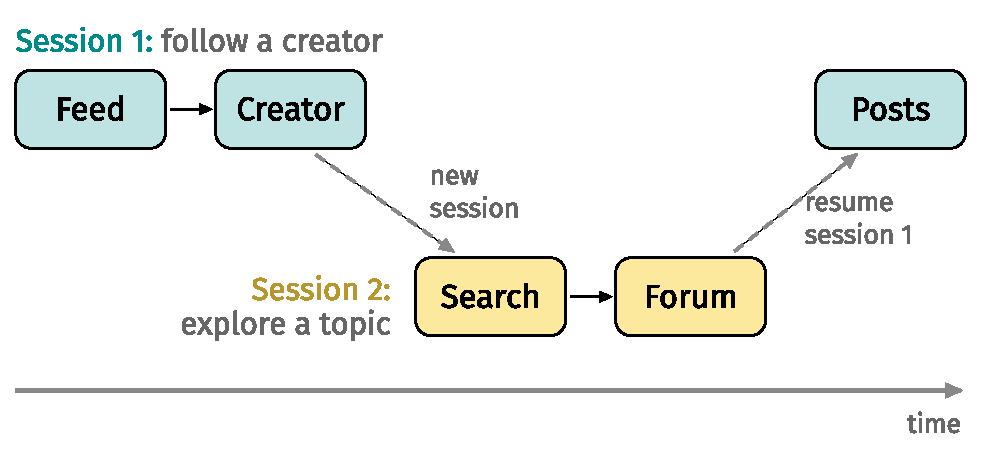
\includegraphics[width=\linewidth]{images/logical-sessions.pdf}
        \end{column}

        \begin{column}{0.4\textwidth}
            \begin{itemize}
                \item Switch probability per sequence: log-normal, mean 15\% \parencite{meiss_whats_2009}
                \item Switch: new session or resume a previous one (50/50)
                \item No backtracking, balanced template distribution
            \end{itemize}
        \end{column}
    \end{columns}
\end{frame}

\begin{frame}{Simulation Methodology: User Interest Modeling}
    \begin{columns}[T]
        \begin{column}{0.55\textwidth}
            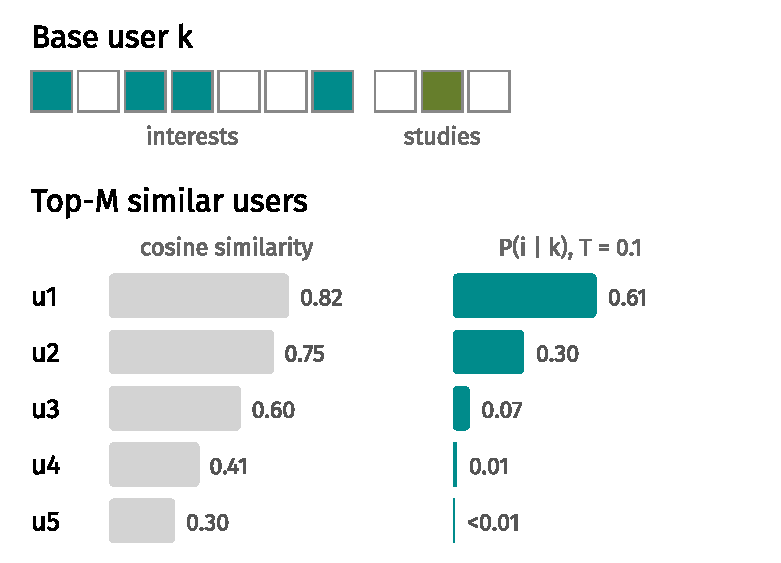
\includegraphics[width=\linewidth]{images/interest-selection.pdf}
        \end{column}

        \begin{column}{0.45\textwidth}
            \begin{itemize}
                \item Binary vector of interests and studies per user
                \item Cosine similarity to base user $k$, keep top-$M$
                \item Softmax selects the first query of each session:
            \end{itemize}
            \[
                P(i \mid k) = \frac{e^{s_{k,i}/T}}{\sum_{u \in C_{k,M}} e^{s_{k,u}/T}}
            \]
        \end{column}
    \end{columns}
\end{frame}

\begin{frame}{Simulation Methodology: Refinement Patterns}
    \centering
    \begin{tabular}{lll}
        \toprule
        \textbf{Behavior} & \textbf{Transformation} & \textbf{Choke points} \\
        \midrule
        Result refinement      & $\pm$ \texttt{FILTER}, $\pm$ selective triple patterns & P.1, P.3 \\
        Result generalization  & $+$ (non-)selective triple patterns                    & P.3, P.4 \\
        Result extension       & $+$ triple patterns, $+$ \texttt{OPTIONAL}/\texttt{UNION} & P.2--P.4 \\
        Query refinement       & $\pm$ \texttt{OPTIONAL}/\texttt{UNION}                 & P.2 \\
        Shifting query intent  & New instantiation values (seeds)                       & T.1, T.2 \\
        \bottomrule
    \end{tabular}

    \vspace{1em}
    \footnotesize
    \begin{tabular}{ll}
        P.1 Filters            & P.2 Filter push-down through \texttt{OPTIONAL}/\texttt{UNION} \\
        P.3 Selective patterns & P.4 Non-selective patterns \\
    \end{tabular}
\end{frame}

\begin{frame}{Simulation Methodology: Refinements Impact Traversal}
    \begin{itemize}\setlength\itemsep{1em}
        \item \textbf{T.1} Predicate additions expand or contract the reachable sub-web
        \item \textbf{T.2} New starting points change the reachable documents
        \item \textbf{T.3} Changes the number of hops to relevant data (SolidBench L.1--L.6)
        \item \textbf{T.4} Alters usability of structural indexes, such as type indexes (L.8)
        \item[$\Rightarrow$] Custom refinement patterns can be defined in JSON
    \end{itemize}
\end{frame}


% NOTES:
% Supplemental slides:
% 
% Examples of discover, short short, short long, complex queries
% Other metrics, such as diefficiency, weighted R^{3} continuos R^{3}?

\end{document}